% !TeX program = pdfLaTeX
\documentclass[12pt]{article}
\usepackage{amsmath}
\usepackage{graphicx,psfrag,epsf}
\usepackage{enumerate}
\usepackage{natbib}
\usepackage{textcomp}
\usepackage[hyphens]{url} % not crucial - just used below for the URL
\usepackage{hyperref}
\providecommand{\tightlist}{%
  \setlength{\itemsep}{0pt}\setlength{\parskip}{0pt}}

%\pdfminorversion=4
% NOTE: To produce blinded version, replace "0" with "1" below.
\newcommand{\blind}{0}

% DON'T change margins - should be 1 inch all around.
\addtolength{\oddsidemargin}{-.5in}%
\addtolength{\evensidemargin}{-.5in}%
\addtolength{\textwidth}{1in}%
\addtolength{\textheight}{1.3in}%
\addtolength{\topmargin}{-.8in}%

%% load any required packages here


\usepackage{color}
\usepackage{fancyvrb}
\newcommand{\VerbBar}{|}
\newcommand{\VERB}{\Verb[commandchars=\\\{\}]}
\DefineVerbatimEnvironment{Highlighting}{Verbatim}{commandchars=\\\{\}}
% Add ',fontsize=\small' for more characters per line
\usepackage{framed}
\definecolor{shadecolor}{RGB}{248,248,248}
\newenvironment{Shaded}{\begin{snugshade}}{\end{snugshade}}
\newcommand{\AlertTok}[1]{\textcolor[rgb]{0.94,0.16,0.16}{#1}}
\newcommand{\AnnotationTok}[1]{\textcolor[rgb]{0.56,0.35,0.01}{\textbf{\textit{#1}}}}
\newcommand{\AttributeTok}[1]{\textcolor[rgb]{0.77,0.63,0.00}{#1}}
\newcommand{\BaseNTok}[1]{\textcolor[rgb]{0.00,0.00,0.81}{#1}}
\newcommand{\BuiltInTok}[1]{#1}
\newcommand{\CharTok}[1]{\textcolor[rgb]{0.31,0.60,0.02}{#1}}
\newcommand{\CommentTok}[1]{\textcolor[rgb]{0.56,0.35,0.01}{\textit{#1}}}
\newcommand{\CommentVarTok}[1]{\textcolor[rgb]{0.56,0.35,0.01}{\textbf{\textit{#1}}}}
\newcommand{\ConstantTok}[1]{\textcolor[rgb]{0.00,0.00,0.00}{#1}}
\newcommand{\ControlFlowTok}[1]{\textcolor[rgb]{0.13,0.29,0.53}{\textbf{#1}}}
\newcommand{\DataTypeTok}[1]{\textcolor[rgb]{0.13,0.29,0.53}{#1}}
\newcommand{\DecValTok}[1]{\textcolor[rgb]{0.00,0.00,0.81}{#1}}
\newcommand{\DocumentationTok}[1]{\textcolor[rgb]{0.56,0.35,0.01}{\textbf{\textit{#1}}}}
\newcommand{\ErrorTok}[1]{\textcolor[rgb]{0.64,0.00,0.00}{\textbf{#1}}}
\newcommand{\ExtensionTok}[1]{#1}
\newcommand{\FloatTok}[1]{\textcolor[rgb]{0.00,0.00,0.81}{#1}}
\newcommand{\FunctionTok}[1]{\textcolor[rgb]{0.00,0.00,0.00}{#1}}
\newcommand{\ImportTok}[1]{#1}
\newcommand{\InformationTok}[1]{\textcolor[rgb]{0.56,0.35,0.01}{\textbf{\textit{#1}}}}
\newcommand{\KeywordTok}[1]{\textcolor[rgb]{0.13,0.29,0.53}{\textbf{#1}}}
\newcommand{\NormalTok}[1]{#1}
\newcommand{\OperatorTok}[1]{\textcolor[rgb]{0.81,0.36,0.00}{\textbf{#1}}}
\newcommand{\OtherTok}[1]{\textcolor[rgb]{0.56,0.35,0.01}{#1}}
\newcommand{\PreprocessorTok}[1]{\textcolor[rgb]{0.56,0.35,0.01}{\textit{#1}}}
\newcommand{\RegionMarkerTok}[1]{#1}
\newcommand{\SpecialCharTok}[1]{\textcolor[rgb]{0.00,0.00,0.00}{#1}}
\newcommand{\SpecialStringTok}[1]{\textcolor[rgb]{0.31,0.60,0.02}{#1}}
\newcommand{\StringTok}[1]{\textcolor[rgb]{0.31,0.60,0.02}{#1}}
\newcommand{\VariableTok}[1]{\textcolor[rgb]{0.00,0.00,0.00}{#1}}
\newcommand{\VerbatimStringTok}[1]{\textcolor[rgb]{0.31,0.60,0.02}{#1}}
\newcommand{\WarningTok}[1]{\textcolor[rgb]{0.56,0.35,0.01}{\textbf{\textit{#1}}}}


\usepackage{float}
\usepackage{xcolor}
\usepackage{booktabs}
\usepackage{longtable}
\usepackage{array}
\usepackage{multirow}
\usepackage{wrapfig}
\usepackage{float}
\usepackage{colortbl}
\usepackage{pdflscape}
\usepackage{tabu}
\usepackage{threeparttable}
\usepackage{threeparttablex}
\usepackage[normalem]{ulem}
\usepackage{makecell}

\begin{document}


\def\spacingset#1{\renewcommand{\baselinestretch}%
{#1}\small\normalsize} \spacingset{1}


%%%%%%%%%%%%%%%%%%%%%%%%%%%%%%%%%%%%%%%%%%%%%%%%%%%%%%%%%%%%%%%%%%%%%%%%%%%%%%

\if0\blind
{
  \title{\bf Classifying ``Fake News'' using Natural Language Processing}

  \author{
        Oliver Baldwin Edwards \\
    Department of Mathematics and Statistics, Amherst College\\
      }
  \maketitle
} \fi

\if1\blind
{
  \bigskip
  \bigskip
  \bigskip
  \begin{center}
    {\LARGE\bf Classifying ``Fake News'' using Natural Language Processing}
  \end{center}
  \medskip
} \fi

\bigskip
\begin{abstract}
Natural Language Processing (NLP) is the process of helping computers
understand and interpret human language (which is hard to do without an
inherent knowledge of tone, connotation, sarcasm, etc.). ``Fake news''
and the validity of news articles, Tweets, and more are at the forefront
of national conversations around free speech and the spread of
misinformation. This project uses NLP to classify news articles as
either real or fake through the use of lemmatization, stop words,
bag-of-words feature extraction, a multilayer perceptron neural network,
a recurrent neural network, and other machine learning models.
\end{abstract}

\noindent%
{\it Keywords:} Natural Language Processing, Fake news, Lemmatization, Bag-of-words, Deep Learning, Recurrent Neural Network
\vfill

\newpage
\spacingset{1.45} % DON'T change the spacing!

\hypertarget{introduction}{%
\section{Introduction}\label{introduction}}

``Fake news'' is a term that has risen to the forefront of the national
conservation over the past few years. According to a 2019 Pew Research
Center survey,\footnote{\citet{mitchellManyAmericansSay2019}} Americans
rate fake news as a larger problem than violent crime, climate change,
and racism (among other categories). In addition---according to the same
survey---68\% of Americans say that fake news has a big impact on their
confidence in government. At its core, fake news is simply defined as
news stories that are false or fabricated. Fake news stories can be
``propaganda that {[}are{]} intentionally designed to mislead the
reader'' or ``clickbait'' stories that are designed for ``economic
incentives.''\footnote{\citet{desaiResearchGuidesFake}}

Due to the issue of fake news, verifying the validity of news articles
(fact-checking) has become an increasingly important job for news
network. This can be seen in the last 2020 presidential debate between
Joe Biden and Donald Trump, where multiple news sources (e.g.~the New
York Times\footnote{\citet{shearFactCheckingFinalPresidential2020}})
reported on the validity of each candidate's claims. Websites such as
Snopes\footnote{\citet{Snopes}} and PolitiFact\footnote{\citet{PolitiFact}}
do this fact-checking on a daily basis. The dataset used in this project
comes from the fact-checking website PolitiFact (see Section
\ref{sec:data}).

However, fact-checking is not perfect. There exist limitations from
fact-checking websites like PolitiFact, such as confirmation bias:
``people may not be likely to fact-check a story that aligns with their
pre-existing beliefs.''\footnote{\citet{asrBigDataQuality2019}}
Additionally, manual fact-checking is a time-intensive process. Thus,
there is motivation to provide another source of fake news assessment: a
statistical model that aims to predict fake news using Natural Language
Processing. Designing a model that does so is the goal of this project.

\hypertarget{background}{%
\section{Background}\label{background}}

\hypertarget{natural-language-processing}{%
\subsection{Natural Language
Processing}\label{natural-language-processing}}

Natural Language Processing (NLP) is the process of helping computers
understand and interpret human language (which is hard to do without an
inherent knowledge of tone, connotation, sarcasm, etc.).\footnote{\citet{cybiantNaturalLanguageProcessing}}
NLP is important because it allows computers to read text (or listen to
speech) and interpret what messages are being conveyed. It is used in
tasks such as sentiment analysis, language translation, or---in the case
of fake news---classification.

NLP is advantageous because it is able to analyze language-based data
``in a consistent and unbiased way.''\footnote{\citet{WhatNaturalLanguage}}
Note that the notion of algorithmic bias\footnote{Algorithmic bias
  describes systematic and repeatable errors in a computer system that
  create unfair outcomes, such as privileging one arbitrary group of
  users over others. \citet{AlgorithmicBias2020}} is a complex topic
that is beyond the scope of this project. Thus, for the purposes of this
project, the NLP used assumes unbiased classification. Assuming this
sort of unbiased classification, using NLP to classify fake news is
clearly beneficial.

In this project, NLP is used to extract features from a set of
PolitiFact claims. Those features, and the associated truth rating of
each claim, are then used to fit multiple machine learning algorithms
with the end goal of classifying fake news with a high accuracy. In
order to extract features from text, lemmatization and stop words are
first used to reduce the size of the overall vocabulary. Then, the
bag-of-words model, which is represented by a document-term matrix
(DTM), is used to create a matrix of features.

\hypertarget{reducing-a-vocabulary-with-lemmatization-and-stop-words}{%
\subsubsection{Reducing a Vocabulary with Lemmatization and Stop
Words}\label{reducing-a-vocabulary-with-lemmatization-and-stop-words}}

In NLP, a text corpus refers to the collection of text documents being
used. In the context of this project, the text corpus is all of the
PolitiFact claims used. A vocabulary, in NLP, is then the set of unique
words used in a text corpus.\footnote{\citet{VocabularyNaturalLanguage}}
When extracting features from text in NLP, a common problem is that the
vocabulary is too large. This is due to the fact that many words that
have very similar meanings (such as ``cook'', ``cooks'', and
``cooking'') are each included as a separate word in the vocabulary. In
addition, many words that (in most contexts) don't carry meaning---such
as ``and'', ``of'', and ``the''---significantly increase the vocabulary
length. To combat this, stemming/lemmatization and the removal of stop
words can be used.

Stemming is a process used in NLP that removes the ends of words in
order to get rid of words that have derivational affixes.\footnote{\citet{StemmingLemmatization}}
There are standard stemming libraries that remove endings of words such
as ``-ing'', ``-es'', and ``-ed''. In addition, users can create their
own custom functions to remove endings of words that are not included in
a stemming library. In stemming, the words ``dog'', ``dogs'', and
``dog's'' would all be cut down to the word ``dog''. This helps to
reduce the number of words that are counted in a document. However, a
word such as ``doggie'' would likely be missed by stemming (unless a
custom function had ``-gie'' set to be removed). Because of such
exceptions, lemmatization is used in this project instead of stemming.

Lemmatization has the same end goal of stemming, but uses a vocabulary
of base words (lemmas) that words in a document are matched to (and then
changed to).\footnote{\citet{StemmingLemmatization}} An example of when
lemmatization is preferable over stemming is with a word such as
``better'', which has ``good'' as its lemma. This sort of word would be
missed with stemming, but caught with lemmatization (which would have a
dictionary matching these two words together). Another example of when
lemmatization is preferable over stemming is with the would ``caring''.
Lemmatizing ``caring'' gives us ``care'', but stemming would likely give
you ``car'' (since a stemming function would erroneously try to remove
just the ``-ing''). Lemmatization is useful since it is able to reduce
the vocabulary size by condensing words that have different textual
representations (but are the same words otherwise) into just one word in
a vocabulary.

Stop word removal is the process of removing specified words from a
vocabulary with the goal of reducing the vocabulary size. Stop words are
words such as ``and'', ``the'', and ``as'' that and add noise to NLP
feature extraction and don't provide any interesting insights. Custom
stop words (depending on the context of the problem at hand) can also be
added to a stop words dictionary.

A full working example of how to clean a single text entry to do the
above discussed lemmatization and stop word removal (as well as some
other standard text cleaning operations) can be seen in the code chunk
below. A very similar text cleaning function is used to clean the
PolitiFact claims in this project (and can be seen in Section
\ref{sec:appendix-data}).

\begin{Shaded}
\begin{Highlighting}[]
\CommentTok{# this is our text input }
\NormalTok{trump_claim_raw <-}\StringTok{ "'Trump approval rating    better than Obama  and Reagan at }
\StringTok{            same point in their presidencies.'"}  

\CommentTok{# a function to perform text cleaning}
\NormalTok{clean_text <-}\StringTok{ }\ControlFlowTok{function}\NormalTok{(input_text) \{}
  \CommentTok{# create a list of all of the stop words we want to remove from our corpus}
  \CommentTok{# note that `stopwords("en")` is a pre-defined list of stop words, but we}
  \CommentTok{# can also add custom stop words (here Obama and Reagan are added)}
\NormalTok{  all_stops <-}\StringTok{ }\KeywordTok{c}\NormalTok{(}\StringTok{"Obama"}\NormalTok{, }\StringTok{"Reagan"}\NormalTok{, }\KeywordTok{stopwords}\NormalTok{(}\StringTok{"en"}\NormalTok{))}

  \CommentTok{# remove any punctuation from the text}
\NormalTok{  output_text <-}\StringTok{ }\KeywordTok{removePunctuation}\NormalTok{(input_text) }\OperatorTok\StringTok{ }
\StringTok{    }\CommentTok{# remove our custom list of stop words}
\StringTok{    }\KeywordTok{removeWords}\NormalTok{(all_stops) }\OperatorTok\StringTok{ }
\StringTok{    }\CommentTok{# make all letters lowercase}
\StringTok{    }\KeywordTok{tolower}\NormalTok{() }\OperatorTok\StringTok{ }
\StringTok{    }\CommentTok{# lemmatize the words in the text }
\StringTok{    }\KeywordTok{lemmatize_strings}\NormalTok{() }\OperatorTok\StringTok{ }
\StringTok{    }\CommentTok{# remove any numbers in the text}
\StringTok{    }\KeywordTok{removeNumbers}\NormalTok{() }\OperatorTok\StringTok{ }
\StringTok{    }\CommentTok{# get rid of any extra white space}
\StringTok{    }\KeywordTok{stripWhitespace}\NormalTok{()}
  
  \KeywordTok{return}\NormalTok{(output_text)}
\NormalTok{\}}

\CommentTok{# apply the text cleaning function}
\NormalTok{trump_claim_clean <-}\StringTok{ }\KeywordTok{clean_text}\NormalTok{(trump_claim_raw)}
\CommentTok{# note how "better" becomes good and "presidencies" becomes "presidency"}
\CommentTok{# also notice that "Obama" and "Reagan" were removed}
\NormalTok{trump_claim_clean}
\end{Highlighting}
\end{Shaded}

\begin{verbatim}
## [1] "trump approval rate good point presidency"
\end{verbatim}

\hypertarget{bag-of-words-model-for-feature-extraction}{%
\subsubsection{Bag-of-Words Model for Feature
Extraction}\label{bag-of-words-model-for-feature-extraction}}

\label{sec:bag-of-words}

Once a vocabulary has been created---and its size reduced---features can
be extracted using the bag-of-words model. The bag-of-words model is a
way to extract features from text by describing the occurrence of each
word in the vocabulary within a single document (and discarding any
information about the order of those words).\footnote{\citet{brownleeGentleIntroductionBagofWords2017}}
Each document in a text corpus (each PolitiFact claim) consists of a
score for each word in the vocabulary. In the most simple case, that
score is simply the number of times each word in a document occurs in
the vocabulary. Note that there are many alternative scoring metrics
here, one such being the term frequency-inverse document frequency
(tf-idf).\footnote{Tf-idf is used to increase the weight of terms which
  are specific to a single document (or handful of documents) and
  decrease the weight for terms used in many documents.
  \citet{AnalyzingTextsText2vec}} (Tf-idf is used as the scoring metric
in this project.)

In practice, bag-of-words feature extraction is represented by a
document-term matrix (DTM). A DTM is ``a matrix that describes the
frequency of terms that occur in a collection of documents'' where
``rows correspond to documents in the collection and columns correspond
to terms.''\footnote{\citet{DocumenttermMatrix2020}} To best illustrate
this, an example of creating a DTM (using term frequency to fill in cell
values) with the \texttt{text2vec} package can be seen in the code chunk
below. Here, we can see a basic example of how to extract features from
an initially uncleaned text corpus by first reducing the vocabulary size
and then creating a DTM. The resulting DTM can be seen in Table
\ref{tab:sample-dtm-table}.

\begin{Shaded}
\begin{Highlighting}[]
\CommentTok{# our initial text corpus}
\NormalTok{car_text <-}\StringTok{ }\KeywordTok{rbind.data.frame}\NormalTok{(}\StringTok{"Bob really likes cars"}\NormalTok{, }
                  \StringTok{"Sally really, really does not like cars"}\NormalTok{,}
                  \StringTok{"Sally only likes 3 types of cars"}\NormalTok{)}

\CommentTok{# add unique document ids }
\NormalTok{car_text <-}\StringTok{ }\KeywordTok{cbind}\NormalTok{(car_text, }\KeywordTok{c}\NormalTok{(}\DecValTok{1}\NormalTok{, }\DecValTok{2}\NormalTok{, }\DecValTok{3}\NormalTok{))}
\KeywordTok{colnames}\NormalTok{(car_text) <-}\StringTok{ }\KeywordTok{c}\NormalTok{(}\StringTok{"text"}\NormalTok{, }\StringTok{"id"}\NormalTok{)}

\CommentTok{# clean the text using the same cleaning function from before}
\CommentTok{# in order to reduce the vocabulary size}
\NormalTok{car_text <-}\StringTok{ }\NormalTok{car_text }\OperatorTok\StringTok{ }
\StringTok{  }\KeywordTok{mutate}\NormalTok{(}\DataTypeTok{cleaned_text =} \KeywordTok{clean_text}\NormalTok{(text))}

\CommentTok{# tokenize the text into individual words }
\NormalTok{tokenizer_car <-}\StringTok{ }\KeywordTok{word_tokenizer}\NormalTok{(car_text}\OperatorTok{$}\NormalTok{cleaned_text) }\OperatorTok\StringTok{ }
\StringTok{  }\KeywordTok{itoken}\NormalTok{(}\DataTypeTok{ids =}\NormalTok{ car_text}\OperatorTok{$}\NormalTok{id, }\DataTypeTok{progressbar =} \OtherTok{FALSE}\NormalTok{)}
         
\CommentTok{# create our vocabulary using the tokenized words}
\NormalTok{car_vocabulary <-}\StringTok{ }\KeywordTok{create_vocabulary}\NormalTok{(tokenizer_car) }

\CommentTok{# create a tokenizer using each word in the vocabulary}
\NormalTok{vocabulary_vectorizer <-}\StringTok{ }\KeywordTok{vocab_vectorizer}\NormalTok{(car_vocabulary) }

\CommentTok{# finally, create our DTM}
\NormalTok{car_dtm <-}\StringTok{ }\KeywordTok{create_dtm}\NormalTok{(tokenizer_car, vocabulary_vectorizer)}
\CommentTok{# convert the DTM to a matrix so that we can print it}
\NormalTok{car_dtm <-}\StringTok{ }\KeywordTok{as.matrix}\NormalTok{(car_dtm)}
\end{Highlighting}
\end{Shaded}

\begin{table}[!h]

\caption{\label{tab:sample-dtm-table}An example DTM using a term frequency
             scoring metric}
\centering
\begin{tabular}[t]{l|r|r|r|r|r|r}
\hline
  & bob & type & sally & car & like & really\\
\hline
1 & 1 & 0 & 0 & 1 & 1 & 1\\
\hline
2 & 0 & 0 & 1 & 1 & 1 & 2\\
\hline
3 & 0 & 1 & 1 & 1 & 1 & 0\\
\hline
\end{tabular}
\end{table}

In Table \ref{tab:sample-dtm-table} we observe that the vocabulary in
this example has been trimmed to six words. Words such as ``does'',
``of'', and ``only'' have been removed and words such as ``likes'' have
been lemmatized to ``like''. Each row represents each of document and
each column represents a word in the vocabulary. Each cell tells us how
many times each vocabulary word appears in a specific document. For
example, the first document has one occurrence of ``really'', the second
document has two occurrences, and the third document has none.

\hypertarget{deep-learning-models}{%
\subsection{Deep Learning Models}\label{deep-learning-models}}

\hypertarget{multilayer-perceptrons}{%
\subsubsection{Multilayer Perceptrons}\label{multilayer-perceptrons}}

Deep learning is a subfield of machine learning that is concerned with
artificial neural networks, which are algorithms inspired by the human
brain. Neural networks---which is what deep learning models refer
to---are beneficial because results tend to get better with more data
and larger models (at the expense of computation and run-time). They are
also able to ``perform automatic feature extraction from raw data,''
which makes them well suited to NLP tasks.\footnote{\citet{brownleeWhatDeepLearning2019}}

To understand how neural networks work we must first understand their
building blocks, perceptrons. A perceptron is made up of four parts:
input values, weights and bias, a net input function, and an activation
function. This can be seen illustrated in Figure
\ref{fig:perceptron-ex}.\footnote{\citet{WhatPerceptronSimplilearn}}

\begin{figure}[H]

{\centering 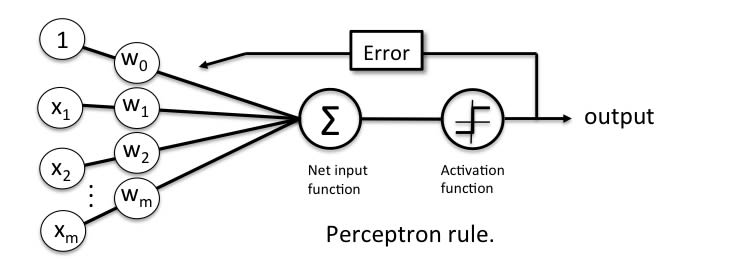
\includegraphics[width=0.9\linewidth,]{images/perceptron-example} 

}

\caption{\label{fig:perceptron-ex}A diagram of a basic perceptron}\label{fig:unnamed-chunk-4}
\end{figure}

The input values, represented by the first row of nodes in the above
figure, are combined with the weight values in the second row of nodes
(weight values are initially randomized). The perceptron then receives
this net input and passes it to the net input function. This net input
is passed to the activation function which decides (based on the net
input) whether or not to generate a \(+1\) or a \(-1\). This generated
output is then the predicted class label of the example. During the
learning phase, the predicted class labels are used to calculate the
error of each prediction and update the weights accordingly.\footnote{\citet{reginaoftechNeuralNetworksBasics2019}}

When more than one perceptron is connected, stacked in several layers, a
neural network is created. In their most basic form, neural networks
consist of an input layer of features, a hidden layer, and an output
layer. A multilayer perceptron (MLP) is a neural network with at least
one hidden layer. Figure \ref{fig:nn-ex} displays a MLP where each node
in the input and hidden layer represent an individual
perceptron.\footnote{\citet{PerceptronsMultiLayerPerceptrons}} Each
perceptron in each layer is connected to every other perceptron in the
following layer with weighted edges. Because there can be a large number
of nodes in each layer, a MLP can quickly become complex. In a similar
way to individual perceptrons, output values are predicted by stepping
through the neural network during the feedforward phase. Edge weights
between neurons are then updated during training through a process
called backpropagation.\footnote{``Backpropagation is an algorithm for
  supervised learning of artificial neural networks using gradient
  descent. Given an artificial neural network and an error function, the
  method calculates the gradient of the error function with respect to
  the neural network's weights.'' \citet{Backpropagation}} This
feedforward and backpropogation process repeats for a user-defined
number of times. Normally, when evaluating a neural network, you should
repeat this process until the edge weights are able to maximize
classification accuracy on a validation set.

\begin{figure}[H]

{\centering 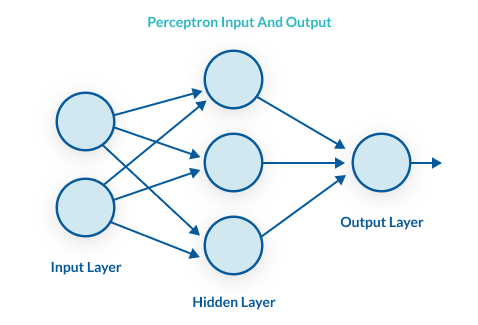
\includegraphics[width=0.7\linewidth,]{images/neural-network-example} 

}

\caption{\label{fig:nn-ex}A diagram of a multilayer perceptron}\label{fig:unnamed-chunk-5}
\end{figure}

Setting the number of hidden layers in a MLP (as well as the number of
nodes in each hidden layer) is an issue of model tuning and can vary
from model to model. However, there is rarely much practical need to
have more than two hidden layers, and one is sufficient in most
problems.\footnote{\citet{ModelSelectionHow}} There is no rule for how
many nodes each layer should have, but a general rule of thumb is this:
the input layer should have as many nodes as there are features and a
hidden layer should have the average of the number of nodes in the input
layer and the number of nodes in the output layer.

\hypertarget{recurrent-neural-networks}{%
\subsubsection{Recurrent Neural
Networks}\label{recurrent-neural-networks}}

Recurrent neural networks (RNN) are designed for problems with a notion
of sequence and add a representation of memory to a neural network. For
this reason, RNNs are well suited to NLP tasks where the sequencing of
words in a sentence matters. RNNs are able to keep track of sequencing
by allowing neurons to pass values sideways within a given layer (in
addition to being able pass values forwards as normal).\footnote{\citet{brownleeCrashCourseRecurrent2016}}

It's important to note that since RNNs require a notion of sequence, the
bag-of-words model mentioned previously needs to be slightly tweaked. In
RNNs, each word in the vocabulary needs its own individual identifier
(in the form of an integer). Then, after text cleaning, documents are
simply translated from word to (id) number. This can still be
represented by a DTM where the number of columns represents the maximum
number of words found in a document within the text corpus and the
number of rows represents the total number of documents. Each cell value
is filled with the numerical representation of each word in a document
(in the original order they appeared in). If a given document is shorter
than the maximum document length, then 0's are simply added to the end
of it.

\newpage

\hypertarget{data}{%
\section{Data}\label{data}}

\label{sec:data}

The data used in this project comes from PolitiFact, a fact-checking
website. Articles, their claims, and the associated truth-levels of
those claims are web-scraped from PolitiFact by the Discourse Processing
Lab at Simon Fraser University\footnote{\citet{taboadaFakeNewsDetection}}.
The Discourse Processing Lab provides a web-scraping tool for multiple
fact checking websites, including PolitiFact and Snopes. The dataset
web-scraped from PolitiFact was chosen over the one from Snopes due to
the fact that PolitiFact has six levels of truth compared to Snopes'
two. The web-scraping works in two parts: first, information is
downloaded from the selected source such as the claim being assessed,
the assessment of that claim, and all links to articles that are
mentioned in the assessment. (That information is all added to the final
dataset.) Then, the link most likely to contain the article being
labeled/assessed is selected, and the original text from that article is
downloaded and added to the dataset.

The PolitiFact dataset includes columns such as the original PolitiFact
URL, the PolitiFact truth rating, the claim of the article being
assessed, the URL and text from the article where the claim came from,
and the category into which the claim being assessed falls. The levels
of truth are described by PolitiFact as the following:

\begin{itemize}
\tightlist
\item
  \textbf{True (1)}: The statement is accurate and there's nothing
  significant missing.
\item
  \textbf{Mostly True (2)}: The statement is accurate but needs
  clarification or additional information.
\item
  \textbf{Half-True (3)}: The statement is partially accurate but leaves
  out important details or takes things out of context.
\item
  \textbf{Mostly False (4)}: The statement contains an element of truth
  but ignores critical facts that would give a different impression.
\item
  \textbf{False (5)}: The statement is not accurate.
\item
  \textbf{Pants on Fire! (6)}: The statement is not accurate and makes a
  ridiculous claim.
\end{itemize}

To simplify the task of classification in this project, only two of the
above truth levels were used in this project. Specifically, only the
PolitiFact claims rated as ``True'' (\(1\)) or ``Pants on Fire!''
(\(6\)) were used. A process where all ratings from 1-3 were classified
as ``True'' and all ratings from 4-6 were classified as ``False'' was
attempted, but this resulted in worse model performance. More discussion
of this can be found in Section \ref{sec:limitations}.

\hypertarget{data-cleaning}{%
\subsection{Data Cleaning}\label{data-cleaning}}

Each entry in this dataset contains a claim that PolitiFact has assigned
a certain truth value. Since multiple external news articles can discuss
the same claim, there can be a single PolitiFact claim/associated truth
value associated with multiple different articles, and thus multiple
different bodies of text. For example, the first three entries in the
raw dataset are all from the same PolitiFact entry which rates the
phrase \emph{``Trump approval rating better than Obama and Reagan at
same point in their presidencies.''} as Mostly True. The reason there
are three entries from this same PolitiFact article (which are all from
the exact same PolitiFact URL) is because multiple news sources (in this
case Fox, NBC, and FiveThirtyEight) all reported on this claim. In an
effort to cut down on the number of duplicate claims such as these, I
have only kept the top entry from each unique PolitiFact URL (even
though the three articles contain different textual content). The reason
for the removal of duplicate entries is further discussed in Section
\ref{sec:limitations}.

In addition to removing duplicate PolitiFact entries, the two targets of
interest (mentioned in the previous section) were filtered, selected,
and converted to numbers. After this, the remaining data cleaning
involved tidying the text of the claims associated with our different
targets as well as reducing the size of the overall vocabulary of words
(for the sake of bag-of-words feature extraction). In particular, this
involved using basic text-cleaning methodologies (such as removing any
punctuation), removing stop words, and using lemmatization. To see the
full data cleaning done in this project, see Section
\ref{sec:appendix-data}.

\hypertarget{exploratory-data-analysis}{%
\subsection{Exploratory Data Analysis}\label{exploratory-data-analysis}}

After the full text cleaning and vocabulary reduction described
previously (and shown fully in Section \ref{sec:appendix-data}), the
vocabulary has \(806\) terms (across \(1911\) documents). To check if
this text cleaning was done properly, we can compare a few selected
article claim documents before and after they were cleaned:

\begin{verbatim}
## [1] "\"Investigators: Anthony Bourdain was killed by Clinton operatives.\""
\end{verbatim}

\begin{verbatim}
## [1] "investigator anthony bourdain kill clinton operative"
\end{verbatim}

\begin{verbatim}
## [1] "Says that people \"went out in their boats to watch\" Hurricane Harvey."
\end{verbatim}

\begin{verbatim}
## [1] "say people go boat watch hurricane harvey"
\end{verbatim}

Since everything is now working as expected, the final thing to explore
is the most frequently used terms in the vocabulary.\footnote{Note that
  it doesn't make sense to visualize the DTM here because it is far too
  large to fully look at, and DTMs are inherently sparse. The DTMs were
  examined and work properly. They can be seen further in
  \ref{sec:appendix-data}.} To get a sense of the the most frequently
used terms in the vocabulary, Figure \ref{fig:word-freq} displays the
top ten most frequently used words in the PolitiFact text corpus.

\begin{figure}[H]
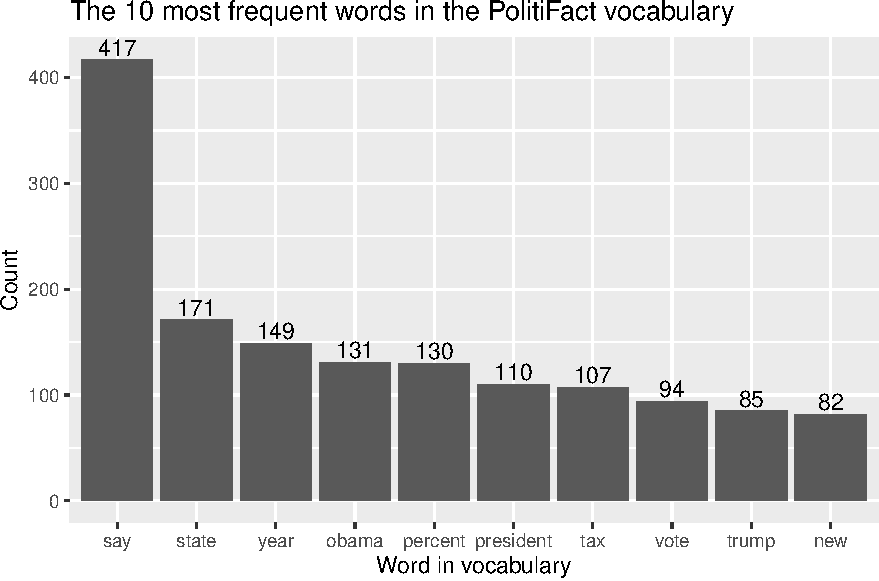
\includegraphics{report_files/figure-latex/word-freq-1} \caption{\label{fig:word-freq}A barplot showing the most frequent words in the PolitiFact vocabulary after text cleaning}\label{fig:word-freq}
\end{figure}

It appears that the word ``say'' was by far the most used word, with
\(417\) occurrences. This is a fairly common word (that is not a stop
word), so this makes sense. It is reasonable to keep ``say'' in this
context as the act of ``stating'' something may be important in
classifying fake news. We also observe that no classic stop word (such
as ``the'') appears in this barplot, which is what we expect. Lastly,
words such as ``obama'', ``president'', and ``trump'' also appear in the
bar plot. Since PolitiFact primarily deals with fact-checking political
claims, this makes sense.

With successful text cleaning and feature extraction, it is time to fit
machine learning models to the data. (Note that the full code for the
process of feature extraction mirrors that of the previous example in
Section \ref{sec:bag-of-words} and can be seen fully in Section
\ref{sec:feature-extraction}.)

\newpage

\newpage

\hypertarget{model-fitting}{%
\section{Model Fitting}\label{model-fitting}}

In this project, seven different machine learning models were fit in an
attempt to classify fake news. The models used were:

\begin{itemize}
\tightlist
\item
  Naive Bayes
\item
  Basic Logistic Regression
\item
  Lasso Regression
\item
  Support Vector Machine
\item
  Random Forest
\item
  Multilayer Perceptron
\item
  Recurrent Neural Network
\end{itemize}

The first five models were fit in order to get a baseline sense of how
non-deep learning algorithms performed when classifying fake news. Then,
the two deep learning models were created in an effort to improve on the
previous models. Since this process requires quite a bit of code as well
as additional explanation for each model, it has been moved to the
Appendix in Section \ref{sec:appendix}. More specifically, the entire
process of model fitting (with code) can be found in Sections
\ref{sec:appendix-initial-models} and
\ref{sec:appendix-deeplearning-models} for the baseline models and deep
learning models respectively.

\newpage

\hypertarget{results}{%
\section{Results}\label{results}}

\begin{table}[!h]

\caption{\label{tab:results-tab}Model accuracies and their corresponding  
             confidence intervals}
\centering
\begin{tabular}[t]{lll}
\toprule
Model & Accuracy & 95\% CI\\
\midrule
\cellcolor{gray!6}{Naive Bayes} & \cellcolor{gray!6}{0.6} & \cellcolor{gray!6}{[0.55, 0.65]}\\
Basic Logistic Regression & 0.62 & [0.57, 0.67]\\
\cellcolor{gray!6}{Lasso Regression} & \cellcolor{gray!6}{0.7} & \cellcolor{gray!6}{[0.65, 0.74]}\\
Support Vector Machine & 0.69 & [0.64, 0.74]\\
\cellcolor{gray!6}{Random Forest} & \cellcolor{gray!6}{0.71} & \cellcolor{gray!6}{[0.66, 0.75]}\\
\addlinespace
Multilayer Perceptron & 0.7 & [0.65, 0.75]\\
\cellcolor{gray!6}{Recurrent Neural Network} & \cellcolor{gray!6}{0.68} & \cellcolor{gray!6}{[0.63, 0.73]}\\
\bottomrule
\end{tabular}
\end{table}

Table \ref{tab:results-tab} displays the resulting accuracies and 95\%
confidence intervals for each of the models run in this project. Basic
approaches, such as Naive Bayes and basic logistic regression performed
noticeably worse than the other five models. It also appears that the
deep learning algorithms did not perform significantly better than any
of the other algorithms (besides Naive Bayes). Note that the confusion
matrices for each of the models can be found in Section
\ref{sec:appendix}.

To examine these results further, we can visualize the confusion matrix
of the random forest model (which did among the best out of all of the
models).

\begin{figure}[H]

{\centering 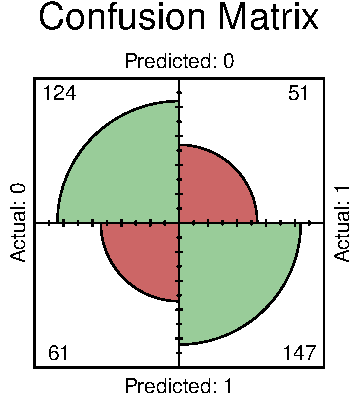
\includegraphics{report_files/figure-latex/unnamed-chunk-7-1} 

}

\caption{\label{fig:conf-mat}Confusion matrix for the random forest model}\label{fig:unnamed-chunk-7}
\end{figure}

Figure \ref{fig:conf-mat} shows that there were 147 true positives, 124
true negatives, 51 false positives, and 61 false negatives. Although the
overall accuracy of around 71\% is not very high, we have a reasonable
balance between the sensitivity and specificity of the predictions.

\newpage

\hypertarget{conclusion}{%
\section{Conclusion}\label{conclusion}}

The goal of this project was to use Natural Language Processing to
classify fake news. To do so, a dataset web scraped from PolitiFact was
used. The text was cleaned, the vocabulary reduced, and features were
extracted. Then, seven different machine learning models were fit using
these features. The two most basic algorithms (Naive Bayes and basic
logistic regression) performed the worst with accuracies of 60\% and
62\% respectively. The other five models performed relatively equally:
they all had accuracies around 70\%.

An automated fake news classifier that performs with a 70\% accuracy is
by no means useless, but it is far from being a robust classifier. With
a topic such as fake news, which has already hurt much of the American
public's perception of the government, any misclassification is
exacerbated. A 70\% accurate fake news classifier used in practice has
poor implications in terms of improving the public's trust in what is
fake and what is not. Thus, far more work is needed in order to create a
reliable fake news classifier. Luckily, there are clear areas in which
this work can be improved upon due to the limitations laid out in the
next section.

\hypertarget{limitations}{%
\subsection{Limitations}\label{limitations}}

\label{sec:limitations}

Among other things, the raw PolitiFact dataset used in this project
contains the original PolitiFact URL, the PolitiFact truth rating, the
claim of the article being assessed, and the URL and text from the
article where the claim came from. The original idea of this project was
to use the original article text (along with the PolitiFact truth
rating) to train a fake news classifier. However, each article's text is
not necessarily making the claim that PolitiFact is grading in each
entry since each PolitiFact grade is based on the claim that an article
is reporting on, and not the article itself.

For example, if an article is reporting on a claim that is false---and
casting the same doubt on that claim that PolitiFact does with their
truth rating of ``False''---then the article text itself is not
necessarily false (even though the claim it's reporting on is). This
means that the target of ``False'' would not be aligned with the article
text. There's no way to check whether or not an article's text is
casting doubt on a claim rather than presenting the same claim that
PolitiFact is fact-checking without manually going through each article.
Since this is infeasible, the project switched from using the original
article text in feature extraction to the claim being graded by
PolitiFact. This meant that duplicate PolitiFact entries could be
removed from the dataset (as they all have the same claim and truth
level).

Additionally, this project initially tried to classify all six different
PolitiFact truth levels. In the end, only the PolitiFact claims rated as
``True'' (\(1\)) or ``Pants on Fire!'' (\(6\)) were used. This was done
as a way to simplify the many models fit in the project as well as to
increase model performance. A process where all ratings from 1-3 were
classified as ``True'' and all ratings from 4-6 were classified as
``False'' was attempted, but this resulted in worse model performance.
The reason for this is likely because article claims are inherently very
short pieces of text and because determining the difference between a
``Half-True'' and ``Mostly False'' article is a very difficult task when
only looking at an article's claim by itself.

The many models fit in this project suffered at the expense of the
amount of data available. After dealing with the limitations mentioned
above, only \(1911\) rows were left in the dataset. This is not nearly
enough data in the context of NLP, especially when using deep learning
algorithms. In standard NLP deep learning problems, datasets have
somewhere on the order of tens of thousands of observations (instead of
\(1911\) in the case of this project).\footnote{\citet{HowBuildNeural}}

\hypertarget{future-work}{%
\subsection{Future Work}\label{future-work}}

The largest areas for future work in this project are to collect more
data and to fine tune the deep learning methods used. As mentioned in
Section \ref{sec:limitations}, the amount of data used in this project
was not on the same scale as other NLP deep learning models. The
collection of more---and higher quality data---is paramount in
increasing the accuracy of a fake news classifier. Additionally, there
is much work to be done to improve the performance of the models used in
this project. A limited amount of hyperparameter tuning was done in this
project, as performing robust hyperparameter tuning for seven different
models is beyond the scope of this project. In particular, there is much
work to be done in fine-tuning the deep learning models due to their
inherent ``black box''\footnote{In machine learning, ``black box''
  refers to the idea that ``data goes in to a model, decisions come out,
  but the processes between input and output are opaque.''
  \citet{BlackBox}} nature.

\newpage

\hypertarget{appendix}{%
\section{Appendix}\label{appendix}}

\label{sec:appendix}

The appendix walks through all of the code performed in this project
including data wrangling, feature extraction, and model fitting.

\hypertarget{data-wranglingfeature-extraction}{%
\subsection{Data Wrangling/Feature
Extraction}\label{data-wranglingfeature-extraction}}

\label{sec:appendix-data}

\hypertarget{basic-data-wrangling}{%
\subsubsection{Basic Data Wrangling}\label{basic-data-wrangling}}

We begin by reading in our raw data:

\begin{Shaded}
\begin{Highlighting}[]
\NormalTok{politifact_df_raw <-}\StringTok{ }\KeywordTok{read_csv}\NormalTok{(}\StringTok{"../data-raw/politifact_phase2_clean_2018_7_3.csv"}\NormalTok{) }
\end{Highlighting}
\end{Shaded}

We then clean up the raw data by getting rid of rows with duplicate
URLs, getting rid of targets we don't care about, and creating two
columns for our targets (one numerical, one categorical) since different
models require different variable types for target values. In addition,
we create a unique ID for each row (which consists of an article's claim
and its PolitiFact truth rating).

\begin{Shaded}
\begin{Highlighting}[]
\CommentTok{# clean up raw data}
\NormalTok{politifact_df_cleaned <-}\StringTok{ }\NormalTok{politifact_df_raw }\OperatorTok\StringTok{ }
\StringTok{  }\CommentTok{# get rid of duplicate URLs (reasoning for this is discussed in limitations)}
\StringTok{  }\KeywordTok{distinct}\NormalTok{(politifact_url_phase1, }\DataTypeTok{.keep_all =} \OtherTok{TRUE}\NormalTok{) }\OperatorTok\StringTok{  }
\StringTok{  }\CommentTok{# keep only the two targets we care about }
\StringTok{  }\KeywordTok{filter}\NormalTok{(fact_tag_phase1 }\OperatorTok{==}\StringTok{ "True"} \OperatorTok{|}\StringTok{ }\NormalTok{fact_tag_phase1 }\OperatorTok{==}\StringTok{ "Pants on Fire!"}\NormalTok{) }\OperatorTok
\StringTok{  }\CommentTok{# change desired targets to categorical and numerical}
\StringTok{  }\KeywordTok{mutate}\NormalTok{(}\DataTypeTok{targets_numerical =} \KeywordTok{as.numeric}\NormalTok{(}\KeywordTok{ifelse}\NormalTok{(fact_tag_phase1 }\OperatorTok{==}\StringTok{ "True"}\NormalTok{, }\DecValTok{1}\NormalTok{, }\DecValTok{0}\NormalTok{)),}
         \DataTypeTok{targets_categorical =} \KeywordTok{as.factor}\NormalTok{(}\KeywordTok{ifelse}\NormalTok{(fact_tag_phase1 }\OperatorTok{==}\StringTok{ "True"}\NormalTok{, }\DecValTok{1}\NormalTok{, }\DecValTok{0}\NormalTok{))) }\OperatorTok
\StringTok{  }\CommentTok{# rename the article claim variable}
\StringTok{  }\KeywordTok{rename}\NormalTok{(}\DataTypeTok{article_claim =}\NormalTok{ article_claim_phase1) }\OperatorTok\StringTok{ }
\StringTok{  }\CommentTok{# only keep the variables we care about}
\StringTok{  }\KeywordTok{select}\NormalTok{(article_claim, targets_numerical, targets_categorical)}

\CommentTok{# add an id }
\NormalTok{politifact_df_cleaned}\OperatorTok{$}\NormalTok{article_id <-}\StringTok{ }\KeywordTok{seq.int}\NormalTok{(}\KeywordTok{nrow}\NormalTok{(politifact_df_cleaned)) }
\CommentTok{# take a look at our cleaned dataframe}
\KeywordTok{glimpse}\NormalTok{(politifact_df_cleaned)}
\end{Highlighting}
\end{Shaded}

\begin{verbatim}
## Rows: 1,911
## Columns: 4
## $ article_claim       <chr> "\"When you tally up their representation in Co...
## $ targets_numerical   <dbl> 1, 0, 0, 0, 1, 0, 1, 0, 1, 0, 1, 1, 0, 0, 1, 0,...
## $ targets_categorical <fct> 1, 0, 0, 0, 1, 0, 1, 0, 1, 0, 1, 1, 0, 0, 1, 0,...
## $ article_id          <int> 1, 2, 3, 4, 5, 6, 7, 8, 9, 10, 11, 12, 13, 14, ...
\end{verbatim}

\hypertarget{cleaning-the-textreducing-the-vocabulary-size}{%
\subsubsection{Cleaning the Text/Reducing the Vocabulary
Size}\label{cleaning-the-textreducing-the-vocabulary-size}}

Since the \texttt{article\_claim} column contains messy text data, text
cleaning is needed. The text cleaning done in this project consists of
the following: removing punctuation, making all letters lowercase,
removing English stop words, lemmatizing each word, removing numbers,
and removing any extra white space. Removing stop words, numbers, and
lemmatizing words all leads to a decrease in the size of the overall
vocabulary (all unique words across a set of text).

The \texttt{clean\_text} function performs the aforementioned text
cleaning and vocabulary reduction:

\begin{Shaded}
\begin{Highlighting}[]
\CommentTok{# a function to perform text cleaning}
\NormalTok{clean_text <-}\StringTok{ }\ControlFlowTok{function}\NormalTok{(input_text) \{}
  \CommentTok{# remove punctuation}
\NormalTok{  output_text <-}\StringTok{ }\KeywordTok{removePunctuation}\NormalTok{(input_text) }\OperatorTok\StringTok{ }
\StringTok{    }\CommentTok{# make all letters lowercase}
\StringTok{    }\KeywordTok{tolower}\NormalTok{() }\OperatorTok\StringTok{ }
\StringTok{    }\CommentTok{# remove a custom list of English stop words (from the `tm` package)}
\StringTok{    }\KeywordTok{removeWords}\NormalTok{(}\KeywordTok{stopwords}\NormalTok{(}\StringTok{"en"}\NormalTok{)) }\OperatorTok\StringTok{ }
\StringTok{    }\CommentTok{# lemmatize the words in the text }
\StringTok{    }\KeywordTok{lemmatize_strings}\NormalTok{() }\OperatorTok\StringTok{ }
\StringTok{    }\CommentTok{# remove any numbers in the text}
\StringTok{    }\KeywordTok{removeNumbers}\NormalTok{() }\OperatorTok\StringTok{ }
\StringTok{    }\CommentTok{# get rid of any extra white space}
\StringTok{    }\KeywordTok{stripWhitespace}\NormalTok{()}
  
  \KeywordTok{return}\NormalTok{(output_text)}
\NormalTok{\}}

\CommentTok{# an example of using the `clean_text` function}
\KeywordTok{clean_text}\NormalTok{(}\StringTok{"'Trump approval rating    better than Obama  and Reagan at }
\StringTok{            same point in their presidencies.'"}\NormalTok{)}
\end{Highlighting}
\end{Shaded}

\begin{verbatim}
## [1] "trump approval rate good obama reagan point presidency"
\end{verbatim}

The \texttt{clean\_text} function is used to clean up the text in
\texttt{politifact\_df\_cleaned}.

\begin{Shaded}
\begin{Highlighting}[]
\CommentTok{# clean up the article claim text, create a final dataframe}
\NormalTok{politifact_df_final <-}\StringTok{ }\NormalTok{politifact_df_cleaned }\OperatorTok\StringTok{ }
\StringTok{  }\KeywordTok{mutate}\NormalTok{(}\DataTypeTok{article_text =} \KeywordTok{clean_text}\NormalTok{(article_claim)) }\OperatorTok\StringTok{ }
\StringTok{  }\KeywordTok{select}\NormalTok{(article_id, article_text, targets_numerical, targets_categorical)}

\KeywordTok{glimpse}\NormalTok{(politifact_df_final) }
\end{Highlighting}
\end{Shaded}

\begin{verbatim}
## Rows: 1,911
## Columns: 4
## $ article_id          <int> 1, 2, 3, 4, 5, 6, 7, 8, 9, 10, 11, 12, 13, 14, ...
## $ article_text        <chr> "tally representation congress governorship dem...
## $ targets_numerical   <dbl> 1, 0, 0, 0, 1, 0, 1, 0, 1, 0, 1, 1, 0, 0, 1, 0,...
## $ targets_categorical <fct> 1, 0, 0, 0, 1, 0, 1, 0, 1, 0, 1, 1, 0, 0, 1, 0,...
\end{verbatim}

\hypertarget{traintest-split}{%
\subsubsection{Train/Test Split}\label{traintest-split}}

In order to evaluate classification models, a training set and a testing
set are needed. In this project, an \(80%
\)/\(20%
\) training/testing split is used.

\begin{Shaded}
\begin{Highlighting}[]
\CommentTok{# set the seed to ensure reproducibility}
\KeywordTok{set.seed}\NormalTok{(}\DecValTok{2}\NormalTok{)}

\CommentTok{# the number of rows in our final data frame }
\NormalTok{num_politifact_rows <-}\StringTok{ }\KeywordTok{nrow}\NormalTok{(politifact_df_final)}

\CommentTok{# get random row numbers from our data frame (80% of all possible row numbers}
\CommentTok{# will be stored in `random_row_numbers` since we have an 80/20 split)}
\NormalTok{random_row_numbers <-}\StringTok{ }\KeywordTok{sample}\NormalTok{(}\DecValTok{1}\OperatorTok{:}\NormalTok{num_politifact_rows, }\FloatTok{0.8} \OperatorTok{*}\StringTok{ }\NormalTok{num_politifact_rows)}

\CommentTok{# use our randomly generated row numbers to select 80% of our data for training}
\NormalTok{politifact_df_train  <-}\StringTok{ }\NormalTok{politifact_df_final[random_row_numbers, ] }\OperatorTok\StringTok{ }
\StringTok{  }\CommentTok{# sort by article id}
\StringTok{  }\KeywordTok{arrange}\NormalTok{(article_id)}
\CommentTok{# and use the remaining 20% of our data for testing}
\NormalTok{politifact_df_test   <-}\StringTok{ }\NormalTok{politifact_df_final[}\OperatorTok{-}\NormalTok{random_row_numbers, ] }\OperatorTok\StringTok{ }
\StringTok{   }\KeywordTok{arrange}\NormalTok{(article_id)}

\CommentTok{# keep track of our target variables in a list }
\NormalTok{train_targets_numerical <-}\StringTok{ }\NormalTok{politifact_df_train}\OperatorTok{$}\NormalTok{targets_numerical}
\NormalTok{train_targets_categorical <-}\StringTok{ }\NormalTok{politifact_df_train}\OperatorTok{$}\NormalTok{targets_categorical}

\NormalTok{test_targets_numerical <-}\StringTok{ }\NormalTok{politifact_df_test}\OperatorTok{$}\NormalTok{targets_numerical}
\NormalTok{test_targets_categorical <-}\StringTok{ }\NormalTok{politifact_df_test}\OperatorTok{$}\NormalTok{targets_categorical}
\end{Highlighting}
\end{Shaded}

We next want to make sure our training/testing split has a roughly equal
distribution of each target value.

\begin{Shaded}
\begin{Highlighting}[]
\KeywordTok{prop.table}\NormalTok{(}\KeywordTok{table}\NormalTok{(train_targets_numerical))}
\end{Highlighting}
\end{Shaded}

\begin{verbatim}
## train_targets_numerical
##         0         1 
## 0.4443717 0.5556283
\end{verbatim}

\begin{Shaded}
\begin{Highlighting}[]
\KeywordTok{prop.table}\NormalTok{(}\KeywordTok{table}\NormalTok{(test_targets_numerical))}
\end{Highlighting}
\end{Shaded}

\begin{verbatim}
## test_targets_numerical
##         0         1 
## 0.4830287 0.5169713
\end{verbatim}

Across our two target variables---where a ``false'' piece of news
corresponds to \(0\) and a ``true'' piece of news corresponds to
\(1\)---we observe a \(44.4%
\), \(55.6%
\) to \(48.3%
\), \(51.7%
\) training/testing split. Since the proportion of target values is
reasonably even, we can proceed with this split.

\hypertarget{creating-a-document-term-matrix}{%
\subsubsection{Creating a Document Term
Matrix}\label{creating-a-document-term-matrix}}

\label{sec:feature-extraction}

To create a Document Term Matrix (DTM), the \texttt{article\_text} needs
to be tokenized into individual words so that an overall vocabulary can
be created. Here n-grams are used (from \(n=1\) to \(n=3\)). This means
that all possible \(1\), \(2\), and \(3\) word combinations are included
in the vocabulary. Note that we must create our vocabulary using only
the training data, since our test data should not be looked at until
model evaluation.

Once a vocabulary is created, terms that only appeared once throughout
our training dataset are removed. This reduces the size of the
vocabulary terms from \(28678\) terms to \(806\), which is a far more
manageable number of terms to have in a DTM.

\begin{Shaded}
\begin{Highlighting}[]
\CommentTok{# tokenize the text into individual words}
\NormalTok{tokenizer_train <-}\StringTok{ }\KeywordTok{word_tokenizer}\NormalTok{(politifact_df_train}\OperatorTok{$}\NormalTok{article_text) }\OperatorTok\StringTok{ }
\StringTok{  }\KeywordTok{itoken}\NormalTok{(}\DataTypeTok{ids =}\NormalTok{ politifact_df_train}\OperatorTok{$}\NormalTok{article_id, }\DataTypeTok{progressbar =} \OtherTok{FALSE}\NormalTok{)}

\CommentTok{# this test tokenizer will be used later}
\NormalTok{tokenizer_test <-}\StringTok{ }\KeywordTok{word_tokenizer}\NormalTok{(politifact_df_test}\OperatorTok{$}\NormalTok{article_text) }\OperatorTok\StringTok{ }
\StringTok{  }\KeywordTok{itoken}\NormalTok{(}\DataTypeTok{ids =}\NormalTok{ politifact_df_test}\OperatorTok{$}\NormalTok{article_id, }\DataTypeTok{progressbar =} \OtherTok{FALSE}\NormalTok{)}
         
\CommentTok{# create our vocabulary with the training data}
\NormalTok{vocabulary <-}\StringTok{ }\KeywordTok{create_vocabulary}\NormalTok{(tokenizer_train, }\DataTypeTok{ngram =} \KeywordTok{c}\NormalTok{(1L, 3L))}
\CommentTok{# we observe 28678 unique terms, this is too large}
\KeywordTok{nrow}\NormalTok{(vocabulary)}
\end{Highlighting}
\end{Shaded}

\begin{verbatim}
## [1] 28678
\end{verbatim}

\begin{Shaded}
\begin{Highlighting}[]
\CommentTok{# prune our vocabulary to only include terms used at least 2 times}
\NormalTok{pruned_vocabulary <-}\StringTok{ }\KeywordTok{prune_vocabulary}\NormalTok{(vocabulary, }\DataTypeTok{term_count_min =} \DecValTok{5}\NormalTok{)}
\CommentTok{# we now observe 806 unique terms, which is more manageable}
\NormalTok{pruned_vocabulary}
\end{Highlighting}
\end{Shaded}

\begin{verbatim}
## Number of docs: 1528 
## 0 stopwords:  ... 
## ngram_min = 1; ngram_max = 3 
## Vocabulary: 
##                 term term_count doc_count
##   1:         account          5         5
##   2:          affair          5         5
##   3:          affect          5         4
##   4: africanamerican          5         5
##   5:           agree          5         5
##  ---                                     
## 802:         percent        130       102
## 803:           obama        131       130
## 804:            year        149       130
## 805:           state        171       159
## 806:             say        417       372
\end{verbatim}

Now that we have a reasonably sized vocabulary, we can create our
training and testing DTMs.

\begin{Shaded}
\begin{Highlighting}[]
\CommentTok{# create our training and testing DTMs using our tokenizers}
\NormalTok{vocabulary_vectorizer <-}\StringTok{ }\KeywordTok{vocab_vectorizer}\NormalTok{(pruned_vocabulary) }

\NormalTok{dtm_train <-}\StringTok{ }\KeywordTok{create_dtm}\NormalTok{(tokenizer_train, vocabulary_vectorizer) }
\NormalTok{dtm_test <-}\StringTok{ }\KeywordTok{create_dtm}\NormalTok{(tokenizer_test, vocabulary_vectorizer)  }
\end{Highlighting}
\end{Shaded}

We then change our DTMs to hold term frequency--inverse document
frequency (tf-idf) values, which will normalize the DTMs and increase
the weight of terms which are specific to a single document (or handful
of documents) and decrease the weight for terms used in many
documents.\footnote{\citet{AnalyzingTextsText2vec}}

\begin{Shaded}
\begin{Highlighting}[]
\NormalTok{tfidf <-}\StringTok{ }\NormalTok{TfIdf}\OperatorTok{$}\KeywordTok{new}\NormalTok{()}

\CommentTok{# fit model to train data and transform train data with fitted model}
\NormalTok{dtm_train <-}\StringTok{  }\KeywordTok{fit_transform}\NormalTok{(dtm_train, tfidf)}
\NormalTok{dtm_test <-}\StringTok{  }\KeywordTok{fit_transform}\NormalTok{(dtm_test, tfidf)}

\CommentTok{# convert our DTMs to a matrix and data frame--different formats are needed}
\CommentTok{# for different models (`keras` only takes matrices for example)}
\NormalTok{dtm_train_matrix <-}\StringTok{ }\KeywordTok{as.matrix}\NormalTok{(dtm_train)}
\NormalTok{dtm_test_matrix <-}\StringTok{ }\KeywordTok{as.matrix}\NormalTok{(dtm_test)}

\NormalTok{dtm_train_df <-}\StringTok{ }\KeywordTok{as.data.frame}\NormalTok{(dtm_train_matrix)}
\NormalTok{dtm_test_df <-}\StringTok{ }\KeywordTok{as.data.frame}\NormalTok{(dtm_test_matrix)}
\end{Highlighting}
\end{Shaded}

The data wrangling and feature extraction is now complete. Our features
exist in the form of Document Term Matrices where each column represents
a term, each row represents a PolitiFact article, and each cell holds
the term frequency--inverse document frequency value of that term. Our
targets exist as \(0\)'s and \(1\)'s, where a ``false'' piece of news
corresponds to 0 and a ``true'' piece of news corresponds to 1. We
observe a small portion of our training and testing DTMs below. Note
that each value is \(0\) since our vocabulary contains \(3000\) terms
and it is very unlikely that the first \(5\) terms are in any of the
\(10\) different rows we are looking at.

\begin{Shaded}
\begin{Highlighting}[]
\NormalTok{dtm_train_df[}\DecValTok{1}\OperatorTok{:}\DecValTok{5}\NormalTok{, }\DecValTok{1}\OperatorTok{:}\DecValTok{5}\NormalTok{]}
\end{Highlighting}
\end{Shaded}

\begin{verbatim}
##   account affair affect africanamerican agree
## 1       0      0      0               0     0
## 3       0      0      0               0     0
## 6       0      0      0               0     0
## 8       0      0      0               0     0
## 9       0      0      0               0     0
\end{verbatim}

\begin{Shaded}
\begin{Highlighting}[]
\NormalTok{dtm_test_df[}\DecValTok{1}\OperatorTok{:}\DecValTok{5}\NormalTok{, }\DecValTok{1}\OperatorTok{:}\DecValTok{5}\NormalTok{]}
\end{Highlighting}
\end{Shaded}

\begin{verbatim}
##    account affair affect africanamerican agree
## 2        0      0      0               0     0
## 4        0      0      0               0     0
## 5        0      0      0               0     0
## 7        0      0      0               0     0
## 12       0      0      0               0     0
\end{verbatim}

\newpage

\hypertarget{initial-model-fitting}{%
\subsection{Initial Model Fitting}\label{initial-model-fitting}}

\label{sec:appendix-initial-models}

This section displays the code for each of the initial models fit in an
attempt to classify fake news.

\hypertarget{naive-bayes}{%
\subsubsection{Naive Bayes}\label{naive-bayes}}

We can use the \texttt{e1071} package to run a Naive Bayes model. Note
that the \texttt{e1071::naiveBayes} function requires categorical
targets and accepts features in the form of a dataframe.

\begin{Shaded}
\begin{Highlighting}[]
\CommentTok{# applying Naive Bayes model to training data}
\NormalTok{nb_model <-}\StringTok{ }\NormalTok{e1071}\OperatorTok{::}\KeywordTok{naiveBayes}\NormalTok{(}\DataTypeTok{x =}\NormalTok{ dtm_train_df, }\DataTypeTok{y =}\NormalTok{ train_targets_categorical, }
                              \DataTypeTok{laplace =} \DecValTok{1}\NormalTok{)}

\CommentTok{# predicting applying to test set}
\NormalTok{nb_predicted_values <-}\StringTok{ }\KeywordTok{predict}\NormalTok{(nb_model, dtm_test_df)}

\NormalTok{nb_confusion_matrix <-}\StringTok{ }\NormalTok{caret}\OperatorTok{::}\KeywordTok{confusionMatrix}\NormalTok{(nb_predicted_values,}
\NormalTok{                                              test_targets_categorical,}
                                              \DataTypeTok{dnn =} \KeywordTok{c}\NormalTok{(}\StringTok{"Predicted"}\NormalTok{, }\StringTok{"Actual"}\NormalTok{)) }
\CommentTok{# confusion matrix table}
\NormalTok{nb_confusion_matrix}\OperatorTok{$}\NormalTok{table}
\end{Highlighting}
\end{Shaded}

\begin{verbatim}
##          Actual
## Predicted   0   1
##         0 137 104
##         1  48  94
\end{verbatim}

\begin{Shaded}
\begin{Highlighting}[]
\CommentTok{# 60.3% accuracy}
\KeywordTok{round}\NormalTok{(nb_confusion_matrix}\OperatorTok{$}\NormalTok{overall[}\DecValTok{1}\NormalTok{], }\DecValTok{3}\NormalTok{)}
\end{Highlighting}
\end{Shaded}

\begin{verbatim}
## Accuracy 
##    0.603
\end{verbatim}

\begin{Shaded}
\begin{Highlighting}[]
\CommentTok{# [55.2%, 65.2%] 95% CI for accuracy}
\KeywordTok{round}\NormalTok{(nb_confusion_matrix}\OperatorTok{$}\NormalTok{overall[}\DecValTok{3}\OperatorTok{:}\DecValTok{4}\NormalTok{], }\DecValTok{3}\NormalTok{)}
\end{Highlighting}
\end{Shaded}

\begin{verbatim}
## AccuracyLower AccuracyUpper 
##         0.552         0.652
\end{verbatim}

\begin{Shaded}
\begin{Highlighting}[]
\CommentTok{# for full information, uncomment and run the following line of code:}
\CommentTok{# nb_confusion_matrix}
\end{Highlighting}
\end{Shaded}

Our Naive Bayes model performs rather poorly with an accuracy of only
\(60.3\%\) (and a 95\% confidence interval of \([55.2\%, 65.2\%]\)).

\hypertarget{basic-logistic-regression}{%
\subsubsection{Basic Logistic
Regression}\label{basic-logistic-regression}}

Since the \texttt{glm} function requires a formula, we must create a new
dataframe combining our features and targets. Note that the \texttt{glm}
function requires categorical targets.

\begin{Shaded}
\begin{Highlighting}[]
\CommentTok{# logistic regression data frames (training and testing)}
\NormalTok{lr_df_train <-}\StringTok{ }\KeywordTok{cbind}\NormalTok{(dtm_train_df, train_targets_categorical)}
\NormalTok{lr_df_test <-}\StringTok{ }\KeywordTok{cbind}\NormalTok{(dtm_test_df, test_targets_categorical)}
\end{Highlighting}
\end{Shaded}

We now fit the logisitic regression model and calculate its accuracy.

\begin{Shaded}
\begin{Highlighting}[]
\CommentTok{# fit the basic logistic regression model}
\NormalTok{blr_model <-}\StringTok{ }\KeywordTok{glm}\NormalTok{(train_targets_categorical }\OperatorTok{~}\StringTok{ }\NormalTok{., }\DataTypeTok{data =}\NormalTok{ lr_df_train,}
                           \DataTypeTok{family =} \KeywordTok{binomial}\NormalTok{(}\DataTypeTok{link =} \StringTok{"logit"}\NormalTok{))}
 
\CommentTok{# calculated the predicted value probabilities (which gives us }
\CommentTok{# the probability that an observation is classified as 1)}
\NormalTok{blr_predicted_value_probs <-}\StringTok{ }\KeywordTok{predict}\NormalTok{(blr_model, }\DataTypeTok{newdata =}\NormalTok{ lr_df_test, }
                                 \DataTypeTok{type =} \StringTok{"response"}\NormalTok{)}

\CommentTok{# turn the probabilites into 1's or 0's--if the probability of being a 1}
\CommentTok{# is greater than 50%, turn it into a 1 (turn it into a 0 otherwise)}
\NormalTok{blr_predicted_values <-}\StringTok{ }\KeywordTok{as.factor}\NormalTok{(}\KeywordTok{ifelse}\NormalTok{(blr_predicted_value_probs }\OperatorTok{>}\StringTok{ }\FloatTok{0.5}\NormalTok{, }\DecValTok{1}\NormalTok{, }\DecValTok{0}\NormalTok{))}

\NormalTok{blr_confusion_matrix <-}\StringTok{ }\NormalTok{caret}\OperatorTok{::}\KeywordTok{confusionMatrix}\NormalTok{(blr_predicted_values,}
\NormalTok{                                               test_targets_categorical,}
                                               \DataTypeTok{dnn =} \KeywordTok{c}\NormalTok{(}\StringTok{"Predicted"}\NormalTok{, }\StringTok{"Actual"}\NormalTok{))}

\CommentTok{# confusion matrix table}
\NormalTok{blr_confusion_matrix}\OperatorTok{$}\NormalTok{table}
\end{Highlighting}
\end{Shaded}

\begin{verbatim}
##          Actual
## Predicted   0   1
##         0 102  63
##         1  83 135
\end{verbatim}

\begin{Shaded}
\begin{Highlighting}[]
\CommentTok{# 61.9% accuracy}
\KeywordTok{round}\NormalTok{(blr_confusion_matrix}\OperatorTok{$}\NormalTok{overall[}\DecValTok{1}\NormalTok{], }\DecValTok{3}\NormalTok{)}
\end{Highlighting}
\end{Shaded}

\begin{verbatim}
## Accuracy 
##    0.619
\end{verbatim}

\begin{Shaded}
\begin{Highlighting}[]
\CommentTok{# [56.8%, 66.8%] 95% CI for accuracy}
\KeywordTok{round}\NormalTok{(blr_confusion_matrix}\OperatorTok{$}\NormalTok{overall[}\DecValTok{3}\OperatorTok{:}\DecValTok{4}\NormalTok{], }\DecValTok{3}\NormalTok{) }
\end{Highlighting}
\end{Shaded}

\begin{verbatim}
## AccuracyLower AccuracyUpper 
##         0.568         0.668
\end{verbatim}

Our basic logistic regression model performs rather poorly with an
accuracy of only \(61.9\%\) (and a 95\% confidence interval of
\([56.8\%, 66.8\%]\)).

\hypertarget{logistic-regresion-with-l1-penalty-lasso-regression}{%
\subsubsection{Logistic Regresion with L1 penalty (Lasso
Regression)}\label{logistic-regresion-with-l1-penalty-lasso-regression}}

This model is an improved form of logistic regression using an L1
regularization penalty and 5-fold cross-validation using the
\texttt{glmnet} package. Logistic regression using an L1 regularization
is also known as ``Lasso regression''. Lasso regression shrinks the less
important features' coefficients to zero, thus removing some features
altogether.\footnote{\citet{nagpalL1L2Regularization2017}} This works
well for feature selection when there are a large number of features, as
in our case (we have \(806\) features).

N-fold cross-validation (here \(n=5\)) is used to ``flag problems like
overfitting or selection bias and to give an insight on how the model
will generalize to an independent dataset.''\footnote{\citet{CrossvalidationStatistics2020}}

The \texttt{cv.glmnet} function from the \texttt{glmnet} function is
used here to perform the Lasso regression and 5-fold cross-validation
discussed above. Note that our features must be in the form of a matrix
here (not a dataframe) and our targets must be numerical.

\begin{Shaded}
\begin{Highlighting}[]
\NormalTok{num_folds <-}\StringTok{ }\DecValTok{5}
\NormalTok{threshold <-}\StringTok{ }\FloatTok{1e-4}
\NormalTok{max_num_it <-}\StringTok{ }\FloatTok{1e5}

\CommentTok{# manually compute our folds so below model doesn't vary each time it's run}
\KeywordTok{set.seed}\NormalTok{(}\DecValTok{2}\NormalTok{)}
\NormalTok{fold_id <-}\StringTok{ }\KeywordTok{sample}\NormalTok{(}\KeywordTok{rep}\NormalTok{(}\KeywordTok{seq}\NormalTok{(num_folds), }\DataTypeTok{length.out =} \KeywordTok{nrow}\NormalTok{(dtm_train_matrix)))}

\CommentTok{# use cross validation to determine the optimal lambda value for L1 penalty}
\NormalTok{lasso_model <-}\StringTok{ }\KeywordTok{cv.glmnet}\NormalTok{(}\DataTypeTok{x =}\NormalTok{ dtm_train_matrix, }\DataTypeTok{y =}\NormalTok{ train_targets_numerical, }
                              \CommentTok{# this gives us logistic regression}
                              \DataTypeTok{family =} \StringTok{"binomial"}\NormalTok{, }
                              \CommentTok{# L1 penalty}
                              \DataTypeTok{alpha =} \DecValTok{1}\NormalTok{,}
                              \CommentTok{# interested in the area under the ROC curve}
                              \DataTypeTok{type.measure =} \StringTok{"auc"}\NormalTok{,}
                              \CommentTok{# 5-fold cross-validation}
                              \DataTypeTok{nfolds =}\NormalTok{ num_folds,}
                              \CommentTok{# manually create our folds for reproducibility}
                              \DataTypeTok{foldid =}\NormalTok{ fold_id,}
                              \CommentTok{# a higher threshold is less accurate, }
                              \CommentTok{# but has faster training}
                              \DataTypeTok{thresh =}\NormalTok{ threshold,}
                              \CommentTok{# a lower number of iterations is less accurate,}
                              \CommentTok{# but has faster training}
                              \DataTypeTok{maxit =}\NormalTok{ max_num_it) }

\NormalTok{lasso_predicted_value_probs <-}\StringTok{ }\KeywordTok{predict}\NormalTok{(lasso_model, dtm_test_matrix, }
                                       \DataTypeTok{type =} \StringTok{"response"}\NormalTok{)}

\NormalTok{lasso_predicted_values <-}\StringTok{ }\KeywordTok{as.factor}\NormalTok{(}\KeywordTok{ifelse}\NormalTok{(lasso_predicted_value_probs }\OperatorTok{>}\StringTok{ }\FloatTok{0.5}\NormalTok{, }\DecValTok{1}\NormalTok{, }\DecValTok{0}\NormalTok{))}

\NormalTok{lasso_confusion_matrix <-}\StringTok{ }\NormalTok{caret}\OperatorTok{::}\KeywordTok{confusionMatrix}\NormalTok{(lasso_predicted_values,}
\NormalTok{                                                 test_targets_categorical,}
                                                 \DataTypeTok{dnn =} \KeywordTok{c}\NormalTok{(}\StringTok{"Predicted"}\NormalTok{, }\StringTok{"Actual"}\NormalTok{))}

\CommentTok{# confusion matrix table}
\NormalTok{lasso_confusion_matrix}\OperatorTok{$}\NormalTok{table}
\end{Highlighting}
\end{Shaded}

\begin{verbatim}
##          Actual
## Predicted   0   1
##         0  91  22
##         1  94 176
\end{verbatim}

\begin{Shaded}
\begin{Highlighting}[]
\CommentTok{# 69.7% accuracy}
\KeywordTok{round}\NormalTok{(lasso_confusion_matrix}\OperatorTok{$}\NormalTok{overall[}\DecValTok{1}\NormalTok{], }\DecValTok{3}\NormalTok{)}
\end{Highlighting}
\end{Shaded}

\begin{verbatim}
## Accuracy 
##    0.697
\end{verbatim}

\begin{Shaded}
\begin{Highlighting}[]
\CommentTok{# [64.8%, 74.3%] 95% CI for accuracy}
\KeywordTok{round}\NormalTok{(lasso_confusion_matrix}\OperatorTok{$}\NormalTok{overall[}\DecValTok{3}\OperatorTok{:}\DecValTok{4}\NormalTok{], }\DecValTok{3}\NormalTok{) }
\end{Highlighting}
\end{Shaded}

\begin{verbatim}
## AccuracyLower AccuracyUpper 
##         0.648         0.743
\end{verbatim}

Our logistic regression model using an L1 regularization penalty
performs significantly better than our basic logistic regression model.
This logistic regression model has an accuracy of \(69.7\%\) (and a 95\%
confidence interval of \([64.8\%, 74.3\%]\)).

\hypertarget{support-vector-machine}{%
\subsubsection{Support Vector Machine}\label{support-vector-machine}}

We can use the \texttt{e1071} package to run a Support Vector Machine
(SVM). Note that the \texttt{randomForest} function requires categorical
targets and accepts features in the form of a dataframe.

\begin{Shaded}
\begin{Highlighting}[]
\NormalTok{svm_model <-}\StringTok{ }\NormalTok{e1071}\OperatorTok{::}\KeywordTok{svm}\NormalTok{(}\DataTypeTok{x =}\NormalTok{ dtm_train_df, }\DataTypeTok{y =}\NormalTok{ train_targets_categorical, }
                        \DataTypeTok{type =} \StringTok{"C-classification"}\NormalTok{, }\DataTypeTok{kernel =} \StringTok{"sigmoid"}\NormalTok{)}
 
\NormalTok{svm_predicted_values <-}\StringTok{ }\KeywordTok{predict}\NormalTok{(svm_model, dtm_test_df)}

\NormalTok{svm_confusion_matrix <-}\StringTok{ }\NormalTok{caret}\OperatorTok{::}\KeywordTok{confusionMatrix}\NormalTok{(svm_predicted_values,}
\NormalTok{                                               test_targets_categorical,}
                                               \DataTypeTok{dnn =} \KeywordTok{c}\NormalTok{(}\StringTok{"Predicted"}\NormalTok{, }\StringTok{"Actual"}\NormalTok{))}

\CommentTok{# confusion matrix table}
\NormalTok{svm_confusion_matrix}\OperatorTok{$}\NormalTok{table}
\end{Highlighting}
\end{Shaded}

\begin{verbatim}
##          Actual
## Predicted   0   1
##         0 113  46
##         1  72 152
\end{verbatim}

\begin{Shaded}
\begin{Highlighting}[]
\CommentTok{# 69.2% accuracy}
\KeywordTok{round}\NormalTok{(svm_confusion_matrix}\OperatorTok{$}\NormalTok{overall[}\DecValTok{1}\NormalTok{], }\DecValTok{3}\NormalTok{)}
\end{Highlighting}
\end{Shaded}

\begin{verbatim}
## Accuracy 
##    0.692
\end{verbatim}

\begin{Shaded}
\begin{Highlighting}[]
\CommentTok{# [64.3%, 73.8%] 95% CI for accuracy}
\KeywordTok{round}\NormalTok{(svm_confusion_matrix}\OperatorTok{$}\NormalTok{overall[}\DecValTok{3}\OperatorTok{:}\DecValTok{4}\NormalTok{], }\DecValTok{3}\NormalTok{) }
\end{Highlighting}
\end{Shaded}

\begin{verbatim}
## AccuracyLower AccuracyUpper 
##         0.643         0.738
\end{verbatim}

Our SVM performs reasonably well with an accuracy of \(69.2\%\) (and a
95\% confidence interval of \([64.3\%, 73.8\%]\)).

\hypertarget{random-forest}{%
\subsubsection{Random Forest}\label{random-forest}}

We can use the \texttt{randomForest} package to run a Naive Bayes model.
Note that the \texttt{randomForest} function requires categorical
targets and accepts features in the form of a dataframe.

\begin{Shaded}
\begin{Highlighting}[]
\KeywordTok{set.seed}\NormalTok{(}\DecValTok{2}\NormalTok{)}
\NormalTok{rf_model <-}\StringTok{ }\KeywordTok{randomForest}\NormalTok{(}\DataTypeTok{x =}\NormalTok{ dtm_train_df, }\DataTypeTok{y =}\NormalTok{ train_targets_categorical)}
\NormalTok{rf_predicted_values <-}\StringTok{ }\KeywordTok{predict}\NormalTok{(rf_model, dtm_test_df)}

\NormalTok{rf_confusion_matrix <-}\StringTok{ }\NormalTok{caret}\OperatorTok{::}\KeywordTok{confusionMatrix}\NormalTok{(rf_predicted_values,}
\NormalTok{                                              test_targets_categorical,}
                                              \DataTypeTok{dnn =} \KeywordTok{c}\NormalTok{(}\StringTok{"Predicted"}\NormalTok{, }\StringTok{"Actual"}\NormalTok{))}

\CommentTok{# confusion matrix table}
\NormalTok{rf_confusion_matrix}\OperatorTok{$}\NormalTok{table}
\end{Highlighting}
\end{Shaded}

\begin{verbatim}
##          Actual
## Predicted   0   1
##         0 124  51
##         1  61 147
\end{verbatim}

\begin{Shaded}
\begin{Highlighting}[]
\CommentTok{# 70.8% accuracy}
\KeywordTok{round}\NormalTok{(rf_confusion_matrix}\OperatorTok{$}\NormalTok{overall[}\DecValTok{1}\NormalTok{], }\DecValTok{3}\NormalTok{)}
\end{Highlighting}
\end{Shaded}

\begin{verbatim}
## Accuracy 
##    0.708
\end{verbatim}

\begin{Shaded}
\begin{Highlighting}[]
\CommentTok{# [65.9%, 75.3%] 95% CI for accuracy}
\KeywordTok{round}\NormalTok{(rf_confusion_matrix}\OperatorTok{$}\NormalTok{overall[}\DecValTok{3}\OperatorTok{:}\DecValTok{4}\NormalTok{], }\DecValTok{3}\NormalTok{) }
\end{Highlighting}
\end{Shaded}

\begin{verbatim}
## AccuracyLower AccuracyUpper 
##         0.659         0.753
\end{verbatim}

Our random forest model performs reasonably well with an accuracy of
\(70.8\%\) (and a 95\% confidence interval of \([65.9\%, 75.3\%]\)).

\newpage

\hypertarget{deep-learning-model-fitting}{%
\subsection{Deep Learning Model
Fitting}\label{deep-learning-model-fitting}}

\label{sec:appendix-deeplearning-models}

This section displays the code for the deep learning models fit in an
attempt to classify fake news.

\hypertarget{multilayer-perceptron-neural-network}{%
\subsubsection{Multilayer Perceptron Neural
Network}\label{multilayer-perceptron-neural-network}}

The \texttt{keras} package is used to fit a Multilayer Perceptron (MLP).
Here, a MLP with one input layer, one hidden layer, and one output layer
is created. The \texttt{keras} requires features to be stored in
matrices and targets to be numerical.

Note that the \texttt{keras} package randomizes initial weights each
time a model is run, meaning that results will vary slightly each time
the following two code chunks are run (specifically, Figure
\ref{fig:mlp-history} will change and the MLP model's accuracy will
change). The provided function to ensure reproducibility in
\texttt{keras}(which is named \texttt{use\_session\_with\_seed()}) does
not currently work within a knitted R Markdown file. Additionally, using
the normal \texttt{set.seed()} function does not alleviate the issue.
For a more detailed breakdown, I've created a file outlining the problem
that can be found in the directory \texttt{scratch-work/keras-reprex.R}.

\begin{Shaded}
\begin{Highlighting}[]
\KeywordTok{set.seed}\NormalTok{(}\DecValTok{2}\NormalTok{)}
\NormalTok{num_features <-}\StringTok{ }\KeywordTok{ncol}\NormalTok{(dtm_train_matrix)}

\CommentTok{# the input layer is implicitly added with input_shape}
\NormalTok{mlp_model <-}\StringTok{ }\KeywordTok{keras_model_sequential}\NormalTok{() }\OperatorTok\StringTok{ }
\StringTok{  }\KeywordTok{layer_dense}\NormalTok{(}\DataTypeTok{units =} \DecValTok{8}\NormalTok{, }\DataTypeTok{activation =} \StringTok{"relu"}\NormalTok{, }\DataTypeTok{input_shape =} \KeywordTok{c}\NormalTok{(num_features)) }\OperatorTok\StringTok{   }
\StringTok{  }\KeywordTok{layer_dense}\NormalTok{(}\DataTypeTok{units =} \DecValTok{1}\NormalTok{, }\DataTypeTok{activation =} \StringTok{"sigmoid"}\NormalTok{)}

\NormalTok{mlp_model }\OperatorTok\StringTok{ }\KeywordTok{compile}\NormalTok{(}
  \DataTypeTok{optimizer =} \StringTok{"rmsprop"}\NormalTok{,}
  \DataTypeTok{loss =} \StringTok{"binary_crossentropy"}\NormalTok{,}
  \DataTypeTok{metrics =} \KeywordTok{c}\NormalTok{(}\StringTok{"accuracy"}\NormalTok{)}
\NormalTok{)}

\CommentTok{# use validation data to determine best number of epochs to run our MLP for}
\NormalTok{mlp_history <-}\StringTok{ }\NormalTok{mlp_model }\OperatorTok\StringTok{ }\NormalTok{keras}\OperatorTok{::}\KeywordTok{fit}\NormalTok{(}
\NormalTok{  dtm_train_matrix, train_targets_numerical,}
  \DataTypeTok{epochs =} \DecValTok{15}\NormalTok{,}
  \DataTypeTok{batch_size =} \DecValTok{1}\NormalTok{,}
  \DataTypeTok{validation_split =} \FloatTok{0.2}
\NormalTok{) }
\end{Highlighting}
\end{Shaded}

\begin{figure}[H]
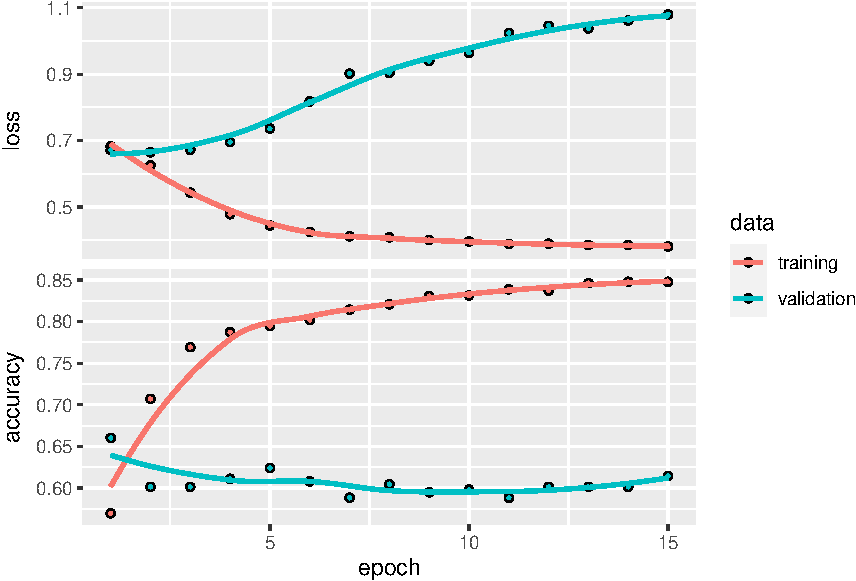
\includegraphics{report_files/figure-latex/unnamed-chunk-25-1} \caption{\label{fig:mlp-history}Validation data performance over multiple epochs in a MLP model}\label{fig:unnamed-chunk-25}
\end{figure}

Figure \ref{fig:mlp-history} shows us how our validation data performs
as our MLP performs multiple feedforward/backpropagation epochs. Since
we want to minimize our validation data's loss and maximize our
validation data's accuracy, we observe that out \(3\) epochs seems to be
reasonable number of times to run our MLP (note that this may change due
to the issue mentioned above about random reproducibility in
\texttt{keras}).

\begin{Shaded}
\begin{Highlighting}[]
\KeywordTok{set.seed}\NormalTok{(}\DecValTok{2}\NormalTok{)}

\NormalTok{mlp_model <-}\StringTok{ }\KeywordTok{keras_model_sequential}\NormalTok{() }\OperatorTok\StringTok{ }
\StringTok{  }\KeywordTok{layer_dense}\NormalTok{(}\DataTypeTok{units =} \DecValTok{8}\NormalTok{, }\DataTypeTok{activation =} \StringTok{"relu"}\NormalTok{, }\DataTypeTok{input_shape =} \KeywordTok{c}\NormalTok{(num_features)) }\OperatorTok\StringTok{   }
\StringTok{  }\KeywordTok{layer_dense}\NormalTok{(}\DataTypeTok{units =} \DecValTok{1}\NormalTok{, }\DataTypeTok{activation =} \StringTok{"sigmoid"}\NormalTok{)}

\NormalTok{mlp_model }\OperatorTok\StringTok{ }\KeywordTok{compile}\NormalTok{(}
  \DataTypeTok{optimizer =} \StringTok{"rmsprop"}\NormalTok{,}
  \DataTypeTok{loss =} \StringTok{"binary_crossentropy"}\NormalTok{,}
  \DataTypeTok{metrics =} \KeywordTok{c}\NormalTok{(}\StringTok{"accuracy"}\NormalTok{)}
\NormalTok{)}
 
\NormalTok{mlp_model }\OperatorTok\StringTok{ }\NormalTok{keras}\OperatorTok{::}\KeywordTok{fit}\NormalTok{(}\DataTypeTok{x =}\NormalTok{ dtm_train_matrix, }\DataTypeTok{y =}\NormalTok{ train_targets_numerical,}
                         \DataTypeTok{epochs =} \DecValTok{3}\NormalTok{, }\DataTypeTok{batch_size =} \DecValTok{1}\NormalTok{)}

\NormalTok{mlp_results <-}\StringTok{ }\NormalTok{mlp_model }\OperatorTok\StringTok{ }\KeywordTok{evaluate}\NormalTok{(}\DataTypeTok{x =}\NormalTok{ dtm_test_matrix, test_targets_numerical)}
\NormalTok{mlp_results}
\end{Highlighting}
\end{Shaded}

\begin{verbatim}
##      loss  accuracy 
## 0.5983205 0.6919060
\end{verbatim}

\begin{Shaded}
\begin{Highlighting}[]
\NormalTok{mlp_predicted_values <-}\StringTok{ }\NormalTok{mlp_model }\OperatorTok\StringTok{ }\KeywordTok{predict_classes}\NormalTok{(dtm_test_matrix, }\DataTypeTok{batch_size =} \DecValTok{1}\NormalTok{)}

\CommentTok{# confusion matrix}
\NormalTok{mlp_confusion_matrix <-}\StringTok{ }\NormalTok{caret}\OperatorTok{::}\KeywordTok{confusionMatrix}\NormalTok{(}\KeywordTok{as.factor}\NormalTok{(mlp_predicted_values),}
\NormalTok{                                              test_targets_categorical,}
                                              \DataTypeTok{dnn =} \KeywordTok{c}\NormalTok{(}\StringTok{"Predicted"}\NormalTok{, }\StringTok{"Actual"}\NormalTok{))}

\CommentTok{# confusion matrix table}
\NormalTok{mlp_confusion_matrix}\OperatorTok{$}\NormalTok{table}
\end{Highlighting}
\end{Shaded}

\begin{verbatim}
##          Actual
## Predicted   0   1
##         0 111  44
##         1  74 154
\end{verbatim}

\begin{Shaded}
\begin{Highlighting}[]
\CommentTok{# around 70% accuracy}
\KeywordTok{round}\NormalTok{(mlp_confusion_matrix}\OperatorTok{$}\NormalTok{overall[}\DecValTok{1}\NormalTok{], }\DecValTok{3}\NormalTok{) }
\end{Highlighting}
\end{Shaded}

\begin{verbatim}
## Accuracy 
##    0.692
\end{verbatim}

\begin{Shaded}
\begin{Highlighting}[]
\CommentTok{# 95% CI}
\KeywordTok{round}\NormalTok{(mlp_confusion_matrix}\OperatorTok{$}\NormalTok{overall[}\DecValTok{3}\OperatorTok{:}\DecValTok{4}\NormalTok{], }\DecValTok{3}\NormalTok{)  }
\end{Highlighting}
\end{Shaded}

\begin{verbatim}
## AccuracyLower AccuracyUpper 
##         0.643         0.738
\end{verbatim}

Our MLP performs reasonably well with an accuracy of around \(70\%\)
(and a 95\% confidence interval around \([65\%, 75\%]\)).

\hypertarget{recurrent-neural-network}{%
\subsubsection{Recurrent Neural
Network}\label{recurrent-neural-network}}

The \texttt{keras} package is used to fit a Recurrent Neural Network
(RNN). Here, a RNN with one input layer, one long short-term memory
(LSTM)\footnote{``LSTMs were developed to deal with the vanishing
  gradient problem that can be encountered when training traditional
  RNNs.'' \citet{LongShorttermMemory2020}} layer, and one output layer
is created. The \texttt{keras} requires features to be stored in
matrices and targets to be numerical. Note that a RNN requires a
different type of DTM representation (as mentioned previously) where
each word must be given a unique numerical ID so that a sense of
sequence can be maintained.

\begin{Shaded}
\begin{Highlighting}[]
\CommentTok{# the number of words to include in our vocab (keep the same as our other vocab)}
\NormalTok{vocab_size <-}\StringTok{ }\DecValTok{806}

\CommentTok{# note that this tokenizer is based on the training data}
\NormalTok{rnn_tokenizer <-}\StringTok{ }\KeywordTok{text_tokenizer}\NormalTok{(}\DataTypeTok{num_words =}\NormalTok{ vocab_size) }\OperatorTok\StringTok{ }
\StringTok{  }\KeywordTok{fit_text_tokenizer}\NormalTok{(politifact_df_train}\OperatorTok{$}\NormalTok{article_text)}

\NormalTok{train_sequences <-}\StringTok{ }\KeywordTok{texts_to_sequences}\NormalTok{(rnn_tokenizer, politifact_df_train}\OperatorTok{$}\NormalTok{article_text)}
\NormalTok{test_sequences <-}\StringTok{ }\KeywordTok{texts_to_sequences}\NormalTok{(rnn_tokenizer, politifact_df_test}\OperatorTok{$}\NormalTok{article_text)}

\CommentTok{# pad sequences (add 0's to the end) for documents that are short}
\NormalTok{rnn_x_train <-}\StringTok{  }\KeywordTok{pad_sequences}\NormalTok{(train_sequences, }\DataTypeTok{padding =} \StringTok{"post"}\NormalTok{)}
\NormalTok{rnn_x_test <-}\StringTok{ }\KeywordTok{pad_sequences}\NormalTok{(test_sequences, }\DataTypeTok{padding =} \StringTok{"post"}\NormalTok{) }

\CommentTok{# take a look at what a RNN DTM looks like}
\NormalTok{rnn_x_train[}\DecValTok{1}\OperatorTok{:}\DecValTok{5}\NormalTok{, }\DecValTok{1}\OperatorTok{:}\DecValTok{5}\NormalTok{]}
\end{Highlighting}
\end{Shaded}

\begin{verbatim}
##      [,1] [,2] [,3] [,4] [,5]
## [1,]   57   48  146  165    3
## [2,]   53  135    0    0    0
## [3,]  219  136    9  368  414
## [4,]    1   11   15  415    0
## [5,]    1  485  137  573   98
\end{verbatim}

Now that we have our features in the right form (they have a notion of
sequence), we can fit our RNN.

\begin{Shaded}
\begin{Highlighting}[]
\KeywordTok{set.seed}\NormalTok{(}\DecValTok{2}\NormalTok{)}

\NormalTok{rnn_model <-}\StringTok{ }\KeywordTok{keras_model_sequential}\NormalTok{()  }\OperatorTok
\StringTok{  }\KeywordTok{layer_embedding}\NormalTok{(}\DataTypeTok{input_dim =}\NormalTok{ vocab_size, }\DataTypeTok{output_dim =} \DecValTok{64}\NormalTok{) }\OperatorTok\StringTok{  }
\StringTok{  }\KeywordTok{layer_lstm}\NormalTok{(}\DataTypeTok{units =} \DecValTok{128}\NormalTok{, }\DataTypeTok{dropout =} \FloatTok{0.2}\NormalTok{, }\DataTypeTok{recurrent_dropout =} \FloatTok{0.2}\NormalTok{) }\OperatorTok\StringTok{ }
\StringTok{  }\KeywordTok{layer_dense}\NormalTok{(}\DataTypeTok{units =} \DecValTok{1}\NormalTok{, }\DataTypeTok{activation =} \StringTok{"sigmoid"}\NormalTok{)}
 
\NormalTok{rnn_model }\OperatorTok\StringTok{ }\KeywordTok{compile}\NormalTok{(}
  \DataTypeTok{optimizer =} \StringTok{"adam"}\NormalTok{,}
  \DataTypeTok{loss =} \StringTok{"binary_crossentropy"}\NormalTok{,}
  \DataTypeTok{metrics =} \KeywordTok{c}\NormalTok{(}\StringTok{"accuracy"}\NormalTok{)}
\NormalTok{)}

\NormalTok{batch_size       <-}\StringTok{ }\DecValTok{64}
\NormalTok{epochs           <-}\StringTok{ }\DecValTok{15}
\NormalTok{validation_split <-}\StringTok{ }\FloatTok{0.1}

\NormalTok{rnn_history <-}\StringTok{ }\NormalTok{rnn_model }\OperatorTok\StringTok{ }\NormalTok{keras}\OperatorTok{::}\KeywordTok{fit}\NormalTok{(}
\NormalTok{  rnn_x_train, train_targets_numerical,}
  \DataTypeTok{batch_size =}\NormalTok{ batch_size,}
  \DataTypeTok{epochs =}\NormalTok{ epochs,}
  \DataTypeTok{validation_split =}\NormalTok{ validation_split}
\NormalTok{)}
\end{Highlighting}
\end{Shaded}

\begin{figure}[H]
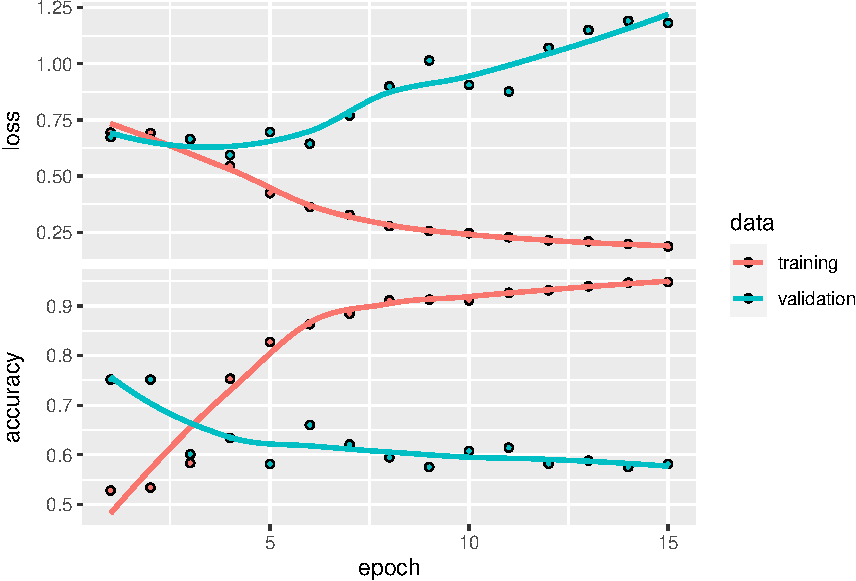
\includegraphics{report_files/figure-latex/unnamed-chunk-29-1} \caption{\label{fig:rnn-history}Validation data performance over multiple epochs in a RNN model}\label{fig:unnamed-chunk-29}
\end{figure}

Figure \ref{fig:rnn-history} shows us how our validation data performs
as our RNN performs multiple feedforward/backpropagation epochs Since we
want to minimize our validation data's loss and maximize our validation
data's accuracy, we observe that out \(3\) epochs seems to be reasonable
number of times to run our MLP (note that this may change due to the
issue mentioned above about random reproducibility in \texttt{keras}).

\begin{Shaded}
\begin{Highlighting}[]
\CommentTok{# recompile model}
\NormalTok{rnn_model <-}\StringTok{ }\KeywordTok{keras_model_sequential}\NormalTok{()  }\OperatorTok
\StringTok{  }\KeywordTok{layer_embedding}\NormalTok{(}\DataTypeTok{input_dim =}\NormalTok{ vocab_size, }\DataTypeTok{output_dim =} \DecValTok{64}\NormalTok{) }\OperatorTok\StringTok{ }
\StringTok{  }\KeywordTok{layer_lstm}\NormalTok{(}\DataTypeTok{units =} \DecValTok{128}\NormalTok{, }\DataTypeTok{dropout =} \FloatTok{0.2}\NormalTok{, }\DataTypeTok{recurrent_dropout =} \FloatTok{0.2}\NormalTok{) }\OperatorTok\StringTok{ }
\StringTok{  }\KeywordTok{layer_dense}\NormalTok{(}\DataTypeTok{units =} \DecValTok{1}\NormalTok{, }\DataTypeTok{activation =} \StringTok{"sigmoid"}\NormalTok{)}
 

\NormalTok{rnn_model }\OperatorTok\StringTok{ }\KeywordTok{compile}\NormalTok{(}
  \DataTypeTok{optimizer =} \StringTok{"adam"}\NormalTok{,}
  \DataTypeTok{loss =} \StringTok{"binary_crossentropy"}\NormalTok{,}
  \DataTypeTok{metrics =} \KeywordTok{c}\NormalTok{(}\StringTok{"accuracy"}\NormalTok{)}
\NormalTok{)}

\NormalTok{rnn_model }\OperatorTok\StringTok{ }\NormalTok{keras}\OperatorTok{::}\KeywordTok{fit}\NormalTok{(rnn_x_train, train_targets_numerical, }\DataTypeTok{epochs =} \DecValTok{3}\NormalTok{, }\DataTypeTok{batch_size =}\NormalTok{ batch_size)}
\NormalTok{rnn_results <-}\StringTok{ }\NormalTok{rnn_model }\OperatorTok\StringTok{ }\KeywordTok{evaluate}\NormalTok{(rnn_x_test, test_targets_numerical)}
\NormalTok{rnn_predicted_values <-}\StringTok{ }\NormalTok{rnn_model }\OperatorTok\StringTok{ }\KeywordTok{predict_classes}\NormalTok{(rnn_x_test, }\DataTypeTok{batch_size =}\NormalTok{ batch_size)}

\CommentTok{# Confusion matrix}
\NormalTok{rnn_confusion_matrix <-}\StringTok{ }\NormalTok{caret}\OperatorTok{::}\KeywordTok{confusionMatrix}\NormalTok{(}\KeywordTok{as.factor}\NormalTok{(rnn_predicted_values),}
\NormalTok{                                              test_targets_categorical,}
                                              \DataTypeTok{dnn =} \KeywordTok{c}\NormalTok{(}\StringTok{"Predicted"}\NormalTok{, }\StringTok{"Actual"}\NormalTok{))}

\CommentTok{# confusion matrix table}
\NormalTok{rnn_confusion_matrix}\OperatorTok{$}\NormalTok{table}
\end{Highlighting}
\end{Shaded}

\begin{verbatim}
##          Actual
## Predicted   0   1
##         0 117  46
##         1  68 152
\end{verbatim}

\begin{Shaded}
\begin{Highlighting}[]
\CommentTok{# around 68% accuracy}
\KeywordTok{round}\NormalTok{(rnn_confusion_matrix}\OperatorTok{$}\NormalTok{overall[}\DecValTok{1}\NormalTok{], }\DecValTok{3}\NormalTok{) }
\end{Highlighting}
\end{Shaded}

\begin{verbatim}
## Accuracy 
##    0.702
\end{verbatim}

\begin{Shaded}
\begin{Highlighting}[]
\CommentTok{# 95% CI  around (0.64, 0.73)}
\KeywordTok{round}\NormalTok{(rnn_confusion_matrix}\OperatorTok{$}\NormalTok{overall[}\DecValTok{3}\OperatorTok{:}\DecValTok{4}\NormalTok{], }\DecValTok{3}\NormalTok{)  }
\end{Highlighting}
\end{Shaded}

\begin{verbatim}
## AccuracyLower AccuracyUpper 
##         0.654         0.748
\end{verbatim}

Our RNN performs reasonably well with an accuracy of around \(68\%\)
(and a 95\% confidence interval around \([63\%, 73\%]\)).

\newpage

\bibliographystyle{agsm}
\bibliography{bibliography.bib}

\end{document}
